%!TEX root = ../thesis.tex
%Adding the above line, with the name of your base .tex file (in this case "thesis.tex") will allow you to compile the whole thesis even when working inside one of the chapter tex files

\singlespacing
\chapter{Conclusions and Future Work} 

\label{chap:6}

\doublespacing
The first goal of this thesis was to derive CME masses from observation with an uncertainty that is the smallest and most reliable to date. This information was then used to calculate a better estimate of CME energies and the first observational quantification of the Lorentz force acting on a CME. 
The second goal of this thesis was to increase the understanding of the relationship between CMEs, CBFs and radio bursts. This was achieved through observational evidence for a CME-driven shock that resulted in a CBF, the acceleration of particles and production of herringbone radio emission. In this chapter, I will summarise and conclude this research and outline the future of this study
\clearpage

\section{CME Masses and Energies}

\subsection{Principle results}

The goal of the this thesis was firstly to derive CME masses from observation that have the smallest and most reliable uncertainty to date. This was achieved using the two vantage points of the \emph{STEREO} Ahead and Behind spacecarft, allowing CME geometry, and the associated mass underestimations, to be fully characterized. This then allowed a better estimate of CME energies and the first observational quantification of the Lorentz force acting on a CME. The principle results are as follows:
\begin{itemize}
\item The first assumption of nearly all CME investigations is that the CME is confined to the 2D sky-plane. This leads to two sources of mass underestimation which primarily arise from the geometrical sensitivity of the Thomson scattering equations for an electron in the solar atmosphere. Firstly, if the CME propagates at some angle away from the sky-plane, but we do not take this angle into account, we will underestimate the mass. Knowledge of the propagation angle from \emph{STEREO} A and B observations allows us to eradicate this uncertainty. The second assumption is that all CME material is confined to a 2D plane at some angle $\theta$. This underestimation cannot be eradicated but we can characterise its effects by simulating a CME with angular width $\psi$ and homogenous density distribution. This allows an estimate of the simulated observed mass and a comparison of this to the actual mass. For any CME width $\psi$ at a sky-plane angle $\theta$ we may calculate the CME mass underestimation when we deproject the CME mass onto its plane $\theta$. A surprising result from this is that for all angular widths $\psi$, deprojection estimates exactly the CME mass when propagation is at an angle $\theta=60^{\circ}$.

\item In the past CME mass uncertainties from the geometrical unknowns described above were either extremely, large at more than 50\% \citep{vou00}, or entirely unquantifiable. Adding to this all the other sources of uncertainty (coronal composition and interactions with streamers) results in CME mass estimates that are entirely unusable in a scientific analysis. In this study, using the capabilities of the STEREO spacecraft, the geometrical mass uncertainties of the CME occurring on 12 December 2008 were reduced to 10\%, a dramatic improvement over previous results. The biggest source of uncertainty was the interaction of this CME with a streamer, adding a further 15\%. Taking everything else into account the final mass uncertainty came to 30\%, which is both smaller and more reliable than any uncertainty given previously. The final total mass of the CME came to
$3.4\pm1.0\times10^{15}$\,g, perhaps the only quotation of mass with an uncertainty in the literature. In an ideal case of a CME that has no background streamer interactions the uncertainty could be reduced even further.

\item This research included the first quantification of the Lorentz force acting on the CME during its early phase propagation. Given $F_{Lorentz} = 3.4\pm2.2\times10^{14}$\,N, it was shown that this is the most dominant force on a CME at $3\,R_{\odot}$, being greater than gravity and drag due to the solar wind. This is the first direct evidence for Lorentz force dominated dynamics, which has been only indirectly shown in previous studies \citep{bein2011}. The quantification of this force is also important for constraining parameters of MHD models of CMEs. There are a variety of models of CMEs which successfully describe the formation of a flux rope and its eruption into interplanetary space (Sections~\ref{sec:cat_model}--\ref{sec:ti_model}). These models employ a number of forces, given by the MHD momentum conservation equation, to propel the CME out of the low corona. The most important of these forces for doing work against the Sun's gravitational potential is the Lorentz ($\mathbf{j}\times\mathbf{B}$) force. While all models include a Lorentz force treated explicitly through currents and magnetic fields, or implicitly only through magnetic fields, the sizes of the force in the models is entirely unconstrained. MHD models of CMEs have the freedom to choose any size Lorentz force because no work had been done on the actual size of this force. For example, \citep{chen1996} predicts a Lorentz force of $\sim$$1.5\times10^{16}$\,N during early phase propagation. This seems to be orders of magnitude too high, and further observational investigations of the forces on CME may show this.

\end{itemize}

\subsection{Future Work}

\subsubsection{CME Mass and Forces Catalogue}

There are a variety of catalogues that list CME kinematical properties for all events detected by space based coronagraphs up to the present time, including the Coordinated Data Analysis Workshop (CDAW) Data Center \citep{gopal2009b}, Computer Aided CME Tracking catalog (CACTus) \citep{robb2004}, Solar Eruptive Event Detection System (SEEDS) \citep{olmedo2008}, and  Automatic Recognition of Transient Events and Marseille Inventory from Synoptic maps (ARTEMIS) \citep{boursier2009}. All of these catalogues provide the speed and acceleration of each CME, however none of them include any estimate of CME mass. The inclusion of CME masses into an entire kinematics catalogue could yield very useful statistical information on CME energies and forces. Such an effort has never been made before, hence there is a need to investigate the feasibility of a kinematics and dynamics catalogue.
\begin{figure}[t!]
\begin{center}
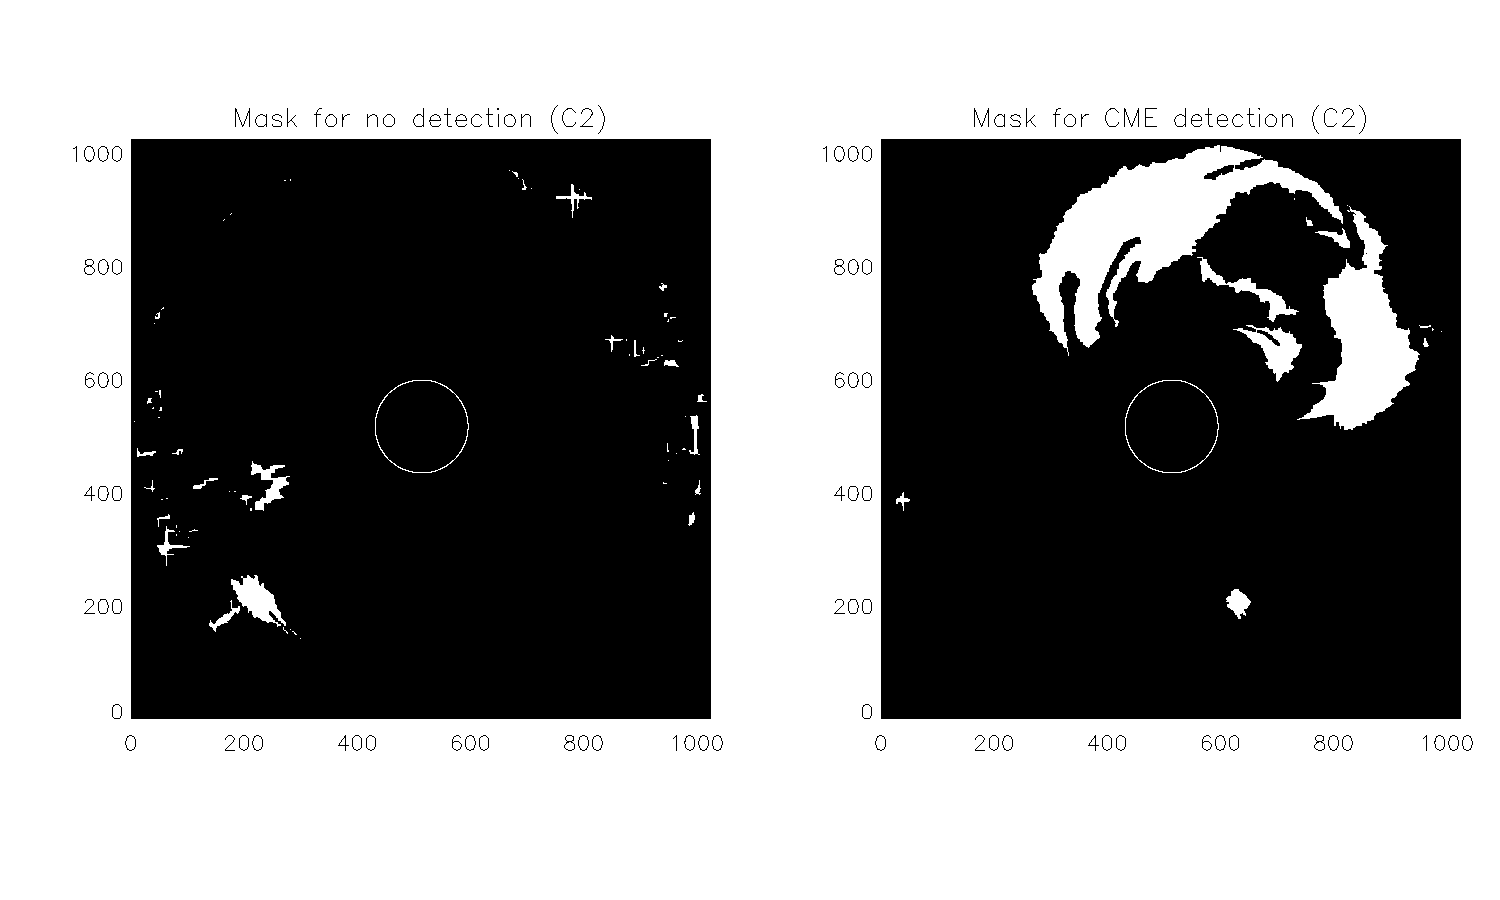
\includegraphics[scale=0.6, trim=2cm 2cm 1cm 1cm]{masks.pdf}
\caption{Sample C2 masks for no-detection (left) and CME-detection (right). Black arrays have a values of 0 and white areas have a value of 1. The no-detection masks has some spurious blobs, possibly due to small ejections of plasma in the solar wind, or cosmic rays on the CCD.}
\label{fig:masks}
\end{center}
\end{figure}

The cataloguing of CME masses is currently being investigated with an automatic tracking tool known as coronal image processing (CORIMP) CME detection \citep{byrne2012}. The CORIMP detection tool is ideal since it uses sophisticated multi-scale analysis techniques to detect only the CME area in the image; isolating the CME area provides the possibility of calculating only the CME mass, without contamination from any other bright features in the image. The product of a CME detection with CORIMP is a mask containing only the area of the image containing the CME. An example of two such masks are shown in Figure~\ref{fig:masks}, with no detection and a CME detection. A conversion of a CME image to pixel values of grams (as described in Chapter 4), application of the detection mask, and summation of all pixels would yield the total mass of the CME. This method was tested on a particularly active period of CME eruptions from 25 April 2010 to 2 May 2010, observed by LASCO C2 and C3. 

%----------------------------------------------------%
%			  Describe method
\begin{figure}[t!]
\begin{center}
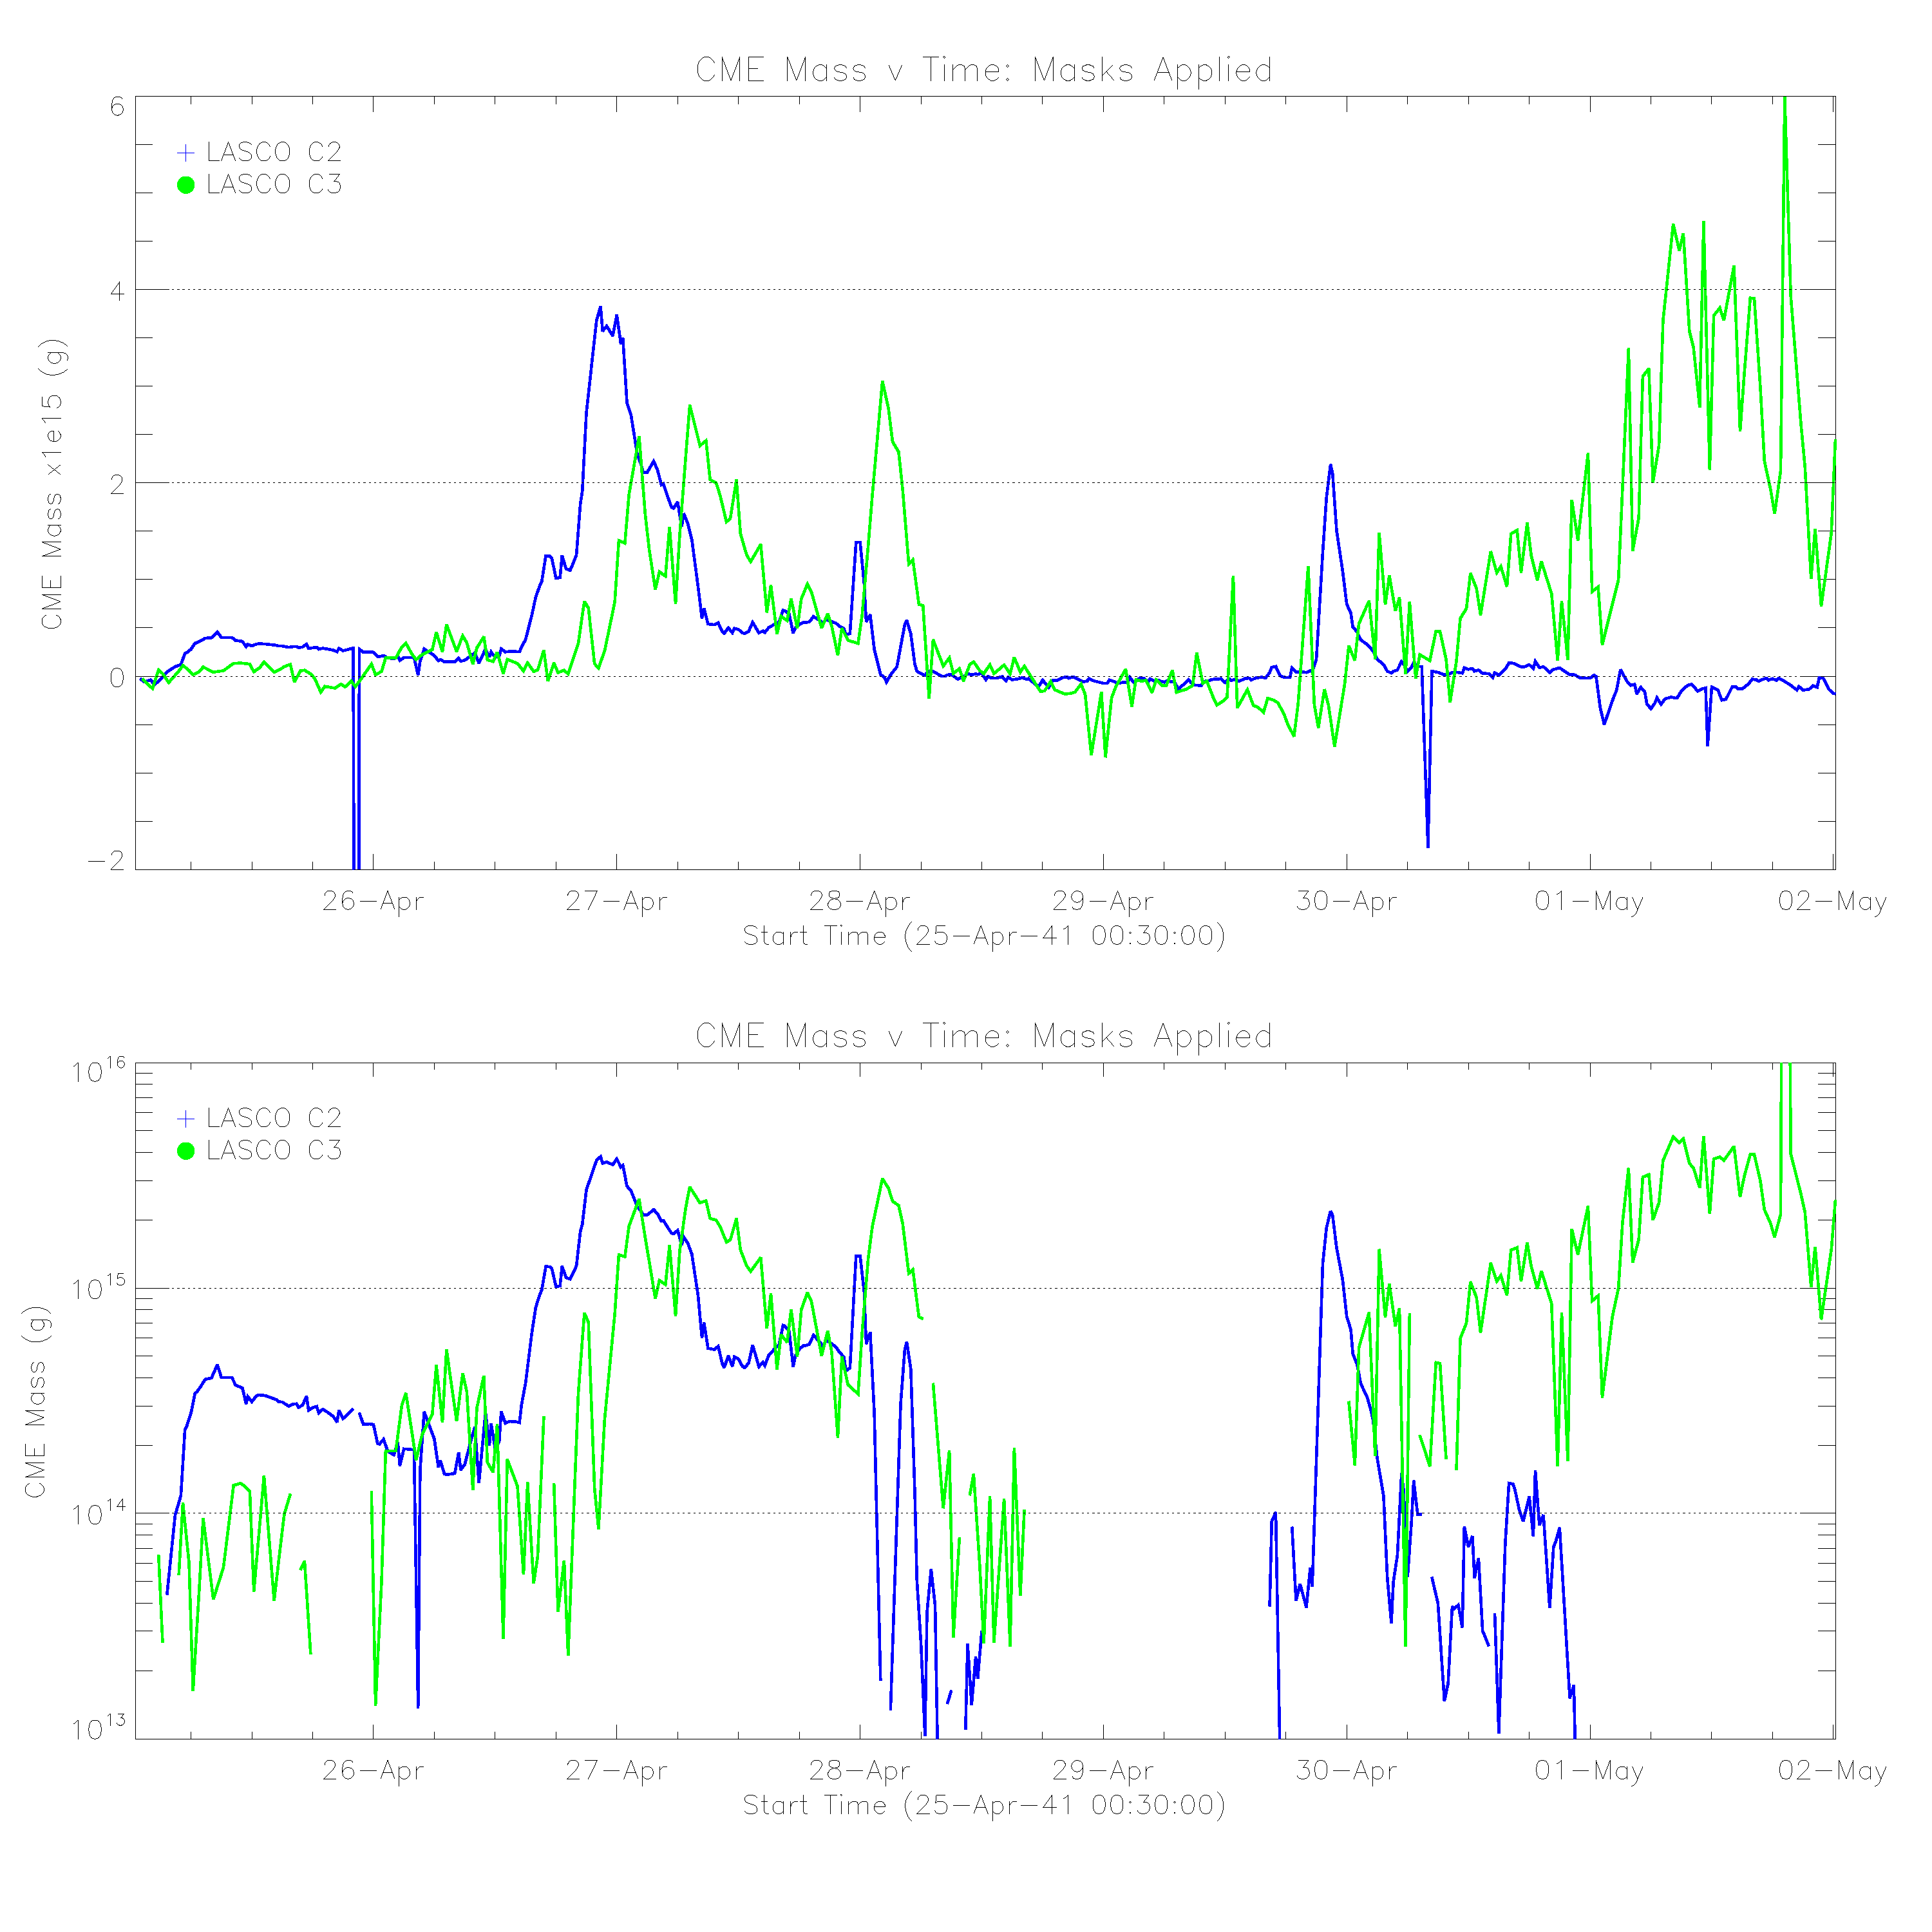
\includegraphics[scale=0.3, trim=7cm 2cm 7cm 4cm]{CME_MASSES_lin_log}
\caption[CME Mass automatic detection]{(Top) Mass estimates calculated using LASCO C2 and C3, and the detection masks of CORIMP. All images in the seven day observation sequence have been base-differenced, with the first image in the sequence used as a pre-event image. Representing mass on a linear scale shows clearly that the method results in reasonable estimates of CME mass. All CMEs are assumed to be propagating on the plane of sky (POS). 
(Bottom) Masses represented on log scale. The CME detection masks tend to capture spurious blobs (mass ejections, but not quite big enough to be regarded as CMEs). These blobs seem to occur in a lot of frames, making the background level sit at $\sim$10$^{14}$\,g or higher. This is a problem if we are to detect small CMEs.}
\label{fig:mass_v_time}
\end{center}
\end{figure}

The detection mask was applied to each image in the sequence between the start and end date. In the majority of images there are no detections (Figure~\ref{fig:masks}(left)) and if a CME is in the image it will be exposed in a mask similar to Figure~\ref{fig:masks}(right). Each image is base-differenced and converted to pixel values of grams using the sky-plane assumption. The pixels are summed such that one image represents one mass value for each image in the sequence i.e., the image sequence allows us to calculate a mass time-series, shown in Figure~\ref{fig:mass_v_time}. The top panel shows a mass time series on a linear scale; the CME detections of a standard $\sim$$10^{15}$\,g can be seen in the time series of both C2 and C3. The method is quite successful in calculating a reasonable mass value for moderate to large CMEs ($\sim$$10^{15}-10^{16}$\,g). 
%----------------------------------------------------%
%			       Initial trial
%

%A more appropriate representation is given in Figure~\ref{fig:mass_v_time}\,(lower), where the y-axis has a log scale. 
Realistically, all of the mass plots should display mass on a log scale, given that CME masses tend to span approximately two orders of magnitude ($10^{14}-10^{16}$\,g). As shown in Figure~\ref{fig:mass_v_time}\,(lower), the log scale reveals a detection of a large background mass even during a quiet period of no CME detection. The background values amount to $\sim$10$^{14}$\,g or slightly higher. This is a problem since small CMEs of $\sim$10$^{14}$\,g will be completely swamped by the background detections, and furthermore, background values may also be misconstrued as legitimate detections. The background values result from an imperfect masking during quiet times. Even though there is no CME, the mask may still detect small clumps and blobs of solar wind that show up as positive areas in the mask Figure~\ref{fig:masks}(left). A current line of investigation to eliminate this is by only accepting detections greater than a certain angular width. Since CMEs tend to be $>40^{\circ}$, anything below this should be rejected and nulled in the mask.
%
%

%
%
%
%----------------------------------------------------%
%	 	Problem with background
%

Other than the spurious detections outlined above, there are a number of tests which need to be performed in order to check that (i) the background subtraction is appropriate (ii) the mask has detected the right quantity of CME mass. 
%At the moment the first image in the observation sequence is subtracted from all subsequent images. However the ideal background image is one just before the eruption takes place.  An algorithm needs to be employed to recognize a period of inactivity prior to eruption, and use an image (or an average of images) from this quiet period in the subsequent base difference.
%----------------------------------------------------%
%	 	 Test of the masking method
%
To check these two criteria we employ the fact that the following must be true
\begin{equation}
M_{mask} = M_{no\_mask} - M_{inverse\_mask}
\end{equation}
where $M_{mass}$ is mass calculated with the mask applied as normal, $M_{no\_mask}$ is just the total image array summed, and $M_{inverse\_mask}$ is the CME masked with the remainder summed. The inverse mask is in Figure~\ref{fig:inverse_masks}. 
\begin{figure}[t!]
\begin{center}
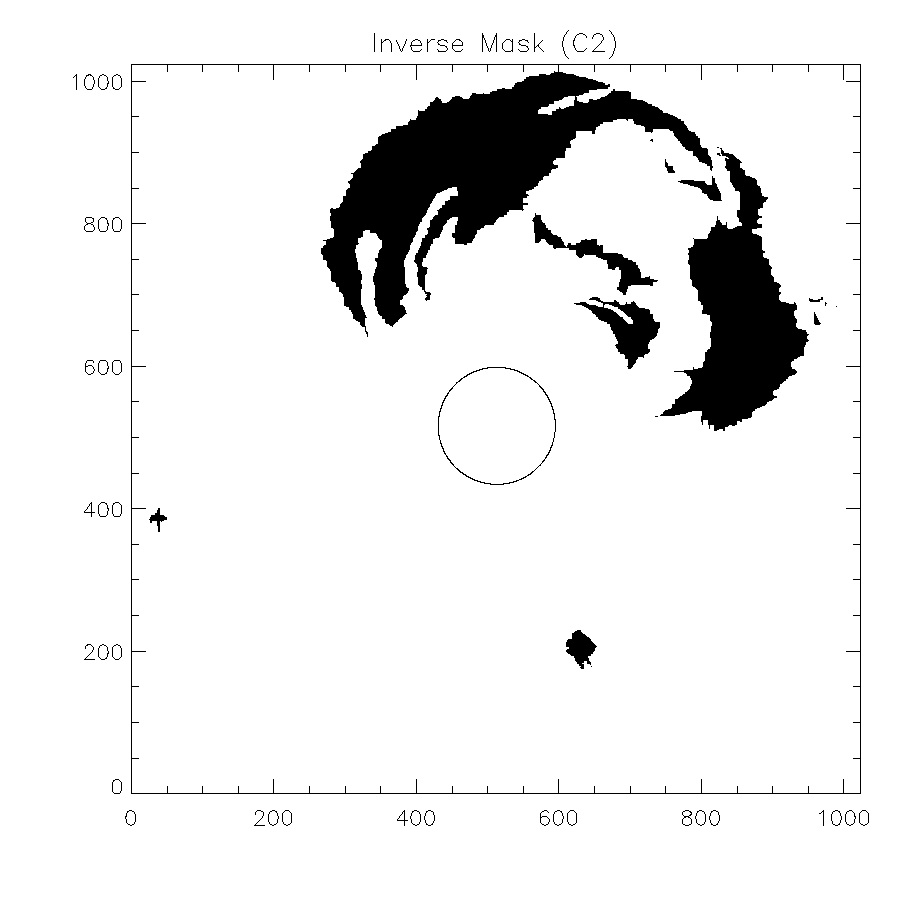
\includegraphics[scale=0.6, trim=0cm 0cm 0cm 0cm]{inverse_masks}
\caption{The inverse mask, with black indicating pixel values of 0 and white indicating values of 1. This allows everything \emph{but} the CME to be summed. Black circle is solar limb.}
\label{fig:inverse_masks}
\end{center}
\end{figure}

\begin{figure}[t!]
\begin{center}
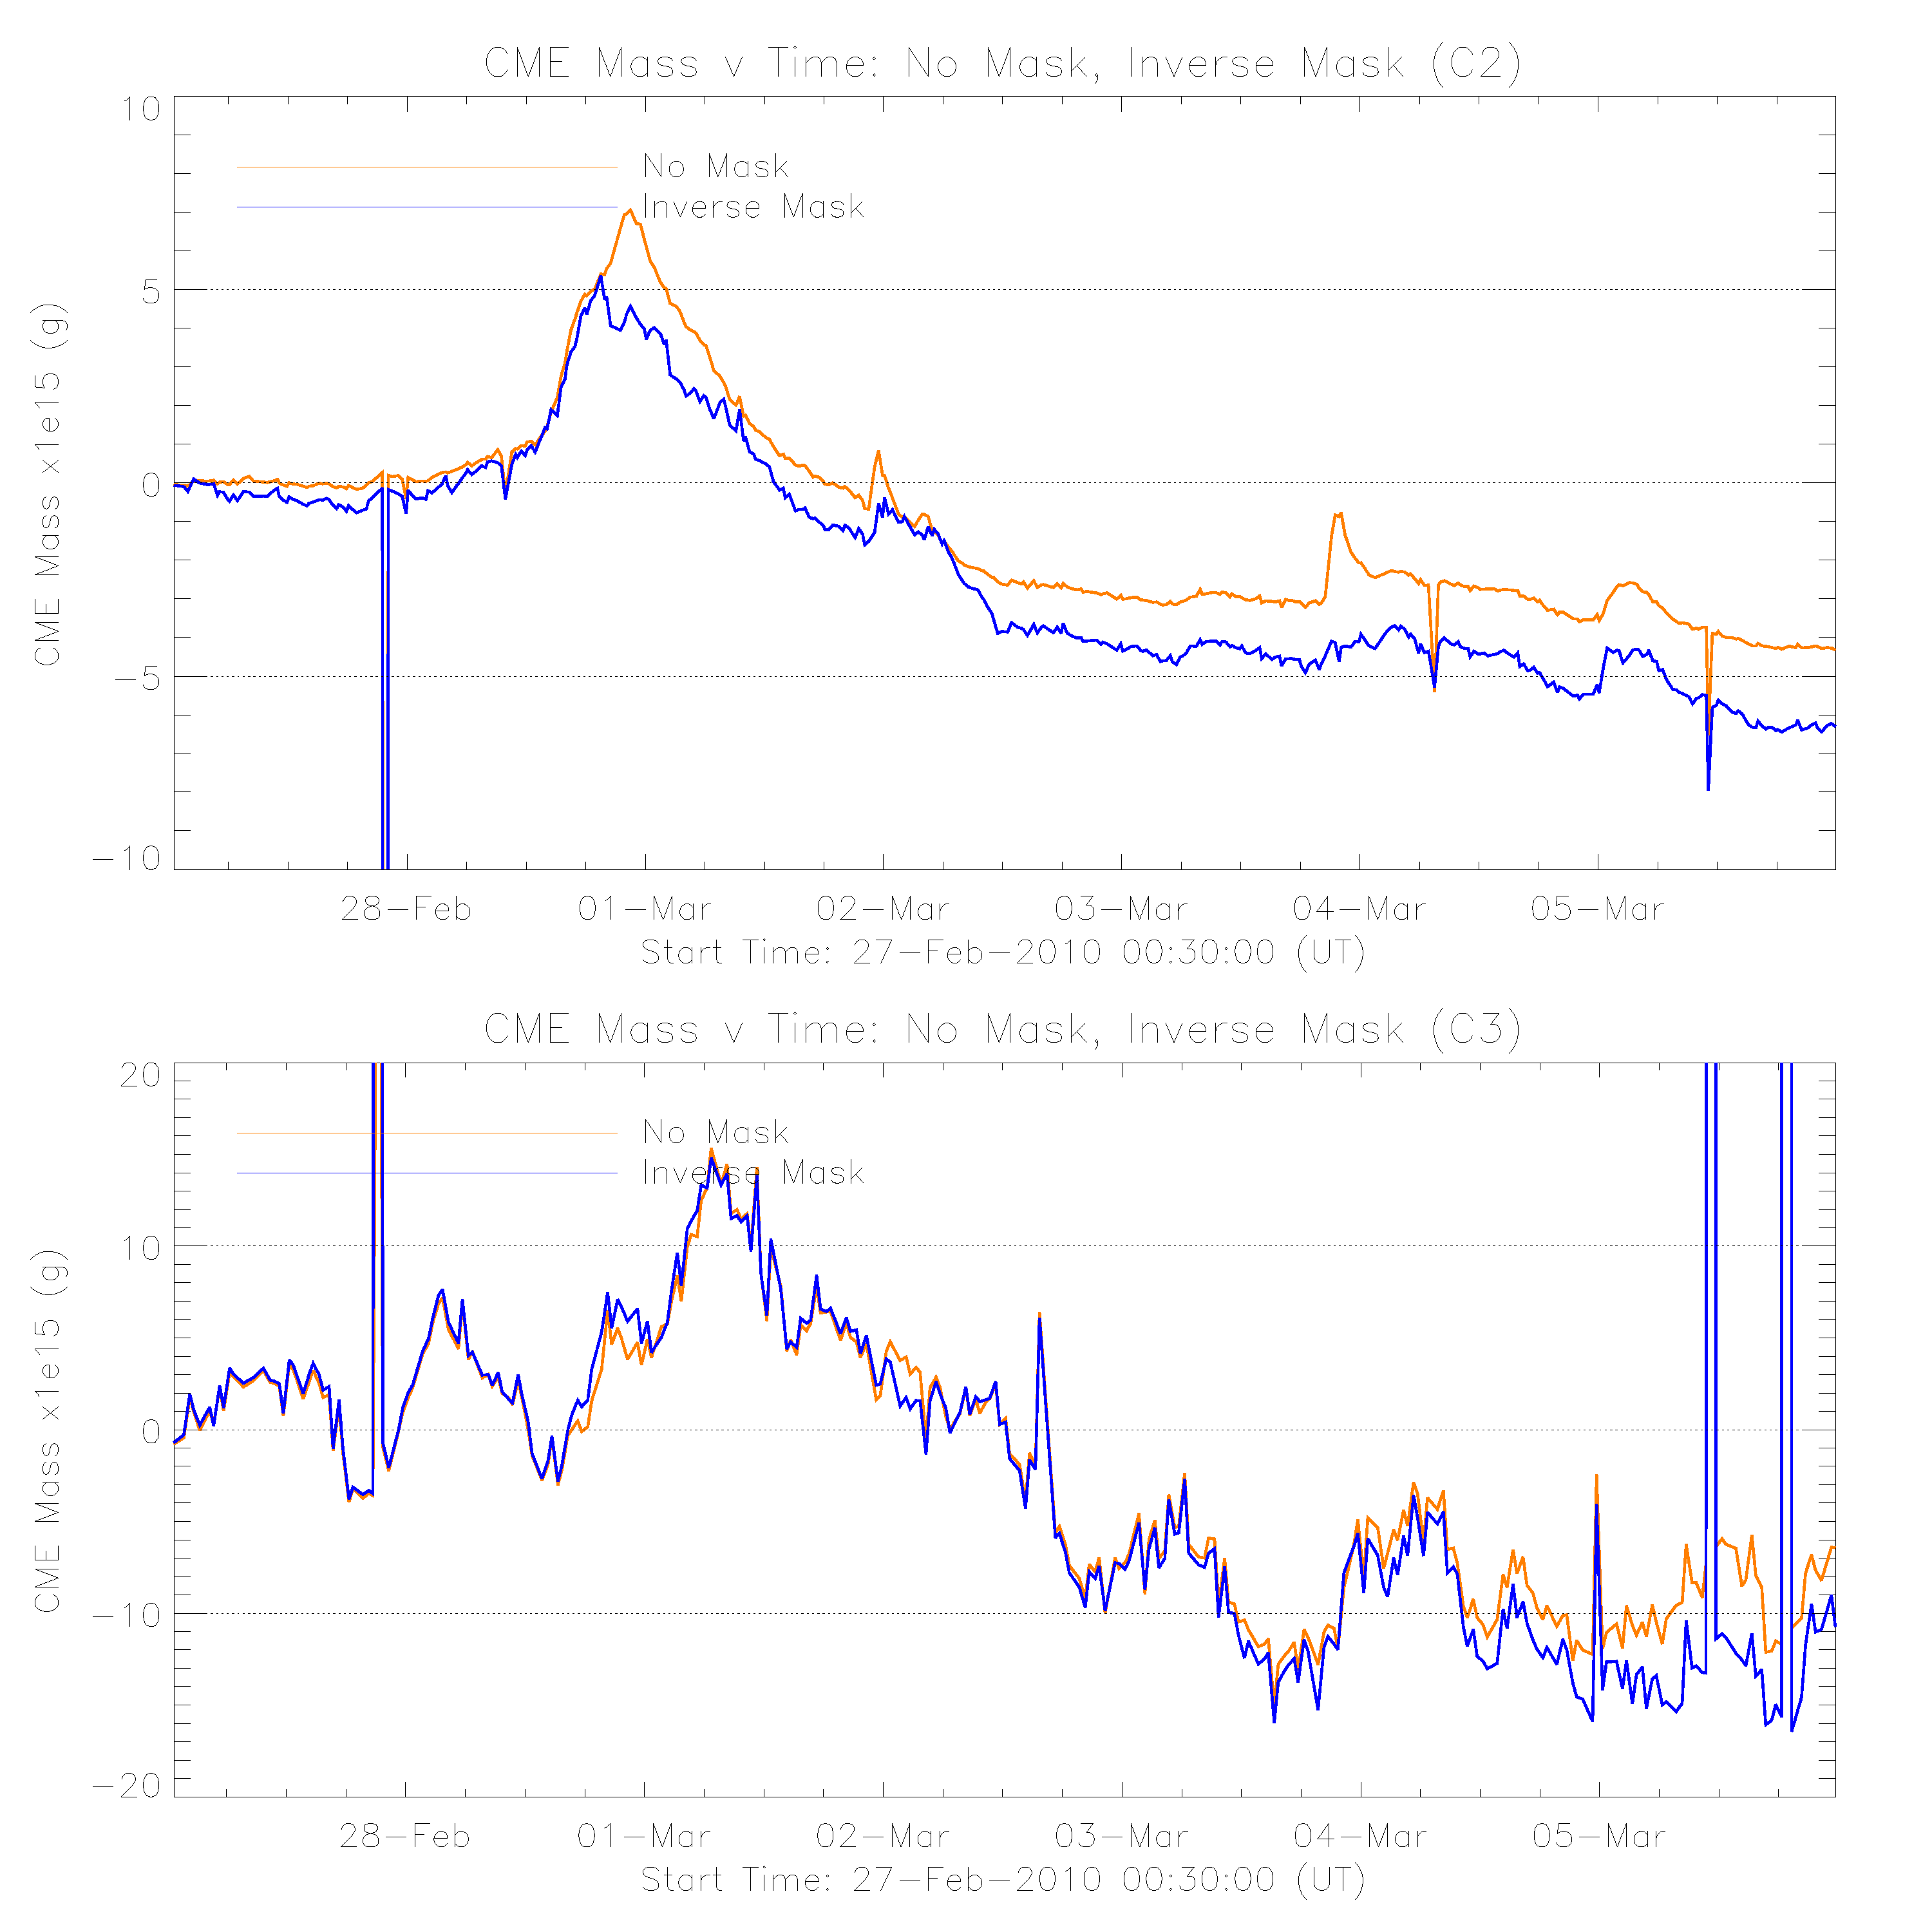
\includegraphics[scale=0.3, trim=0cm 2cm 0cm 1cm]{compare_masks_c2c3}
\caption{Time series of the mass obtained from using no mask and using the inverse mask. The data behave as expected, with the inverse mask being essentially the same as the no-mask but smaller by the CME mass. The drift towards negative values is symptomatic of a pre-event image (for base-difference) that is too bright. The discontinuous values are due to badly prepped images in the NRL archive.}
\label{fig:comparison0}
\end{center}
\end{figure}
We perform the time series again to calculate $M_{no\_mask}$ and $M_{inverse\_mask}$, shown in Figure~\ref{fig:comparison0}. They behave as expected, with the inverse-mask being essentially the same as the no-mask, but smaller by a roughly constant amount; this roughly constant amount should equal the CME mass. The effect of a single pre-event image used in the base-difference for the whole sequence is very apparent. In both C2 and C3 the masses grow toward increasingly negative values. This happens because the pre-event image is too bright and is a bad representation of the background corona over the observation sequences. In the intervening hours between start and end time a number of CMEs erupt. This will result in a dimming of the background corona over time as the corona becomes depleted or evacuated. This method has determined that condition (i) is not fulfilled, and is a good error check to see if an appropriate background has been chosen. An algorithm needs to be employed to recognize a period of inactivity prior to eruption, and use an image (or an average of images) from this quiet period in the subsequent base difference.

To test condition (ii) we compare the difference of the blue and orange time series in Figure~\ref{fig:comparison0} with the time series calculated using the normal mask (Figure~\ref{fig:mass_v_time}), the results are shown in Figure~\ref{fig:comparison}. The trends in both time series match, however they diverge as time increases. 
\begin{figure}[t!]
\begin{center}
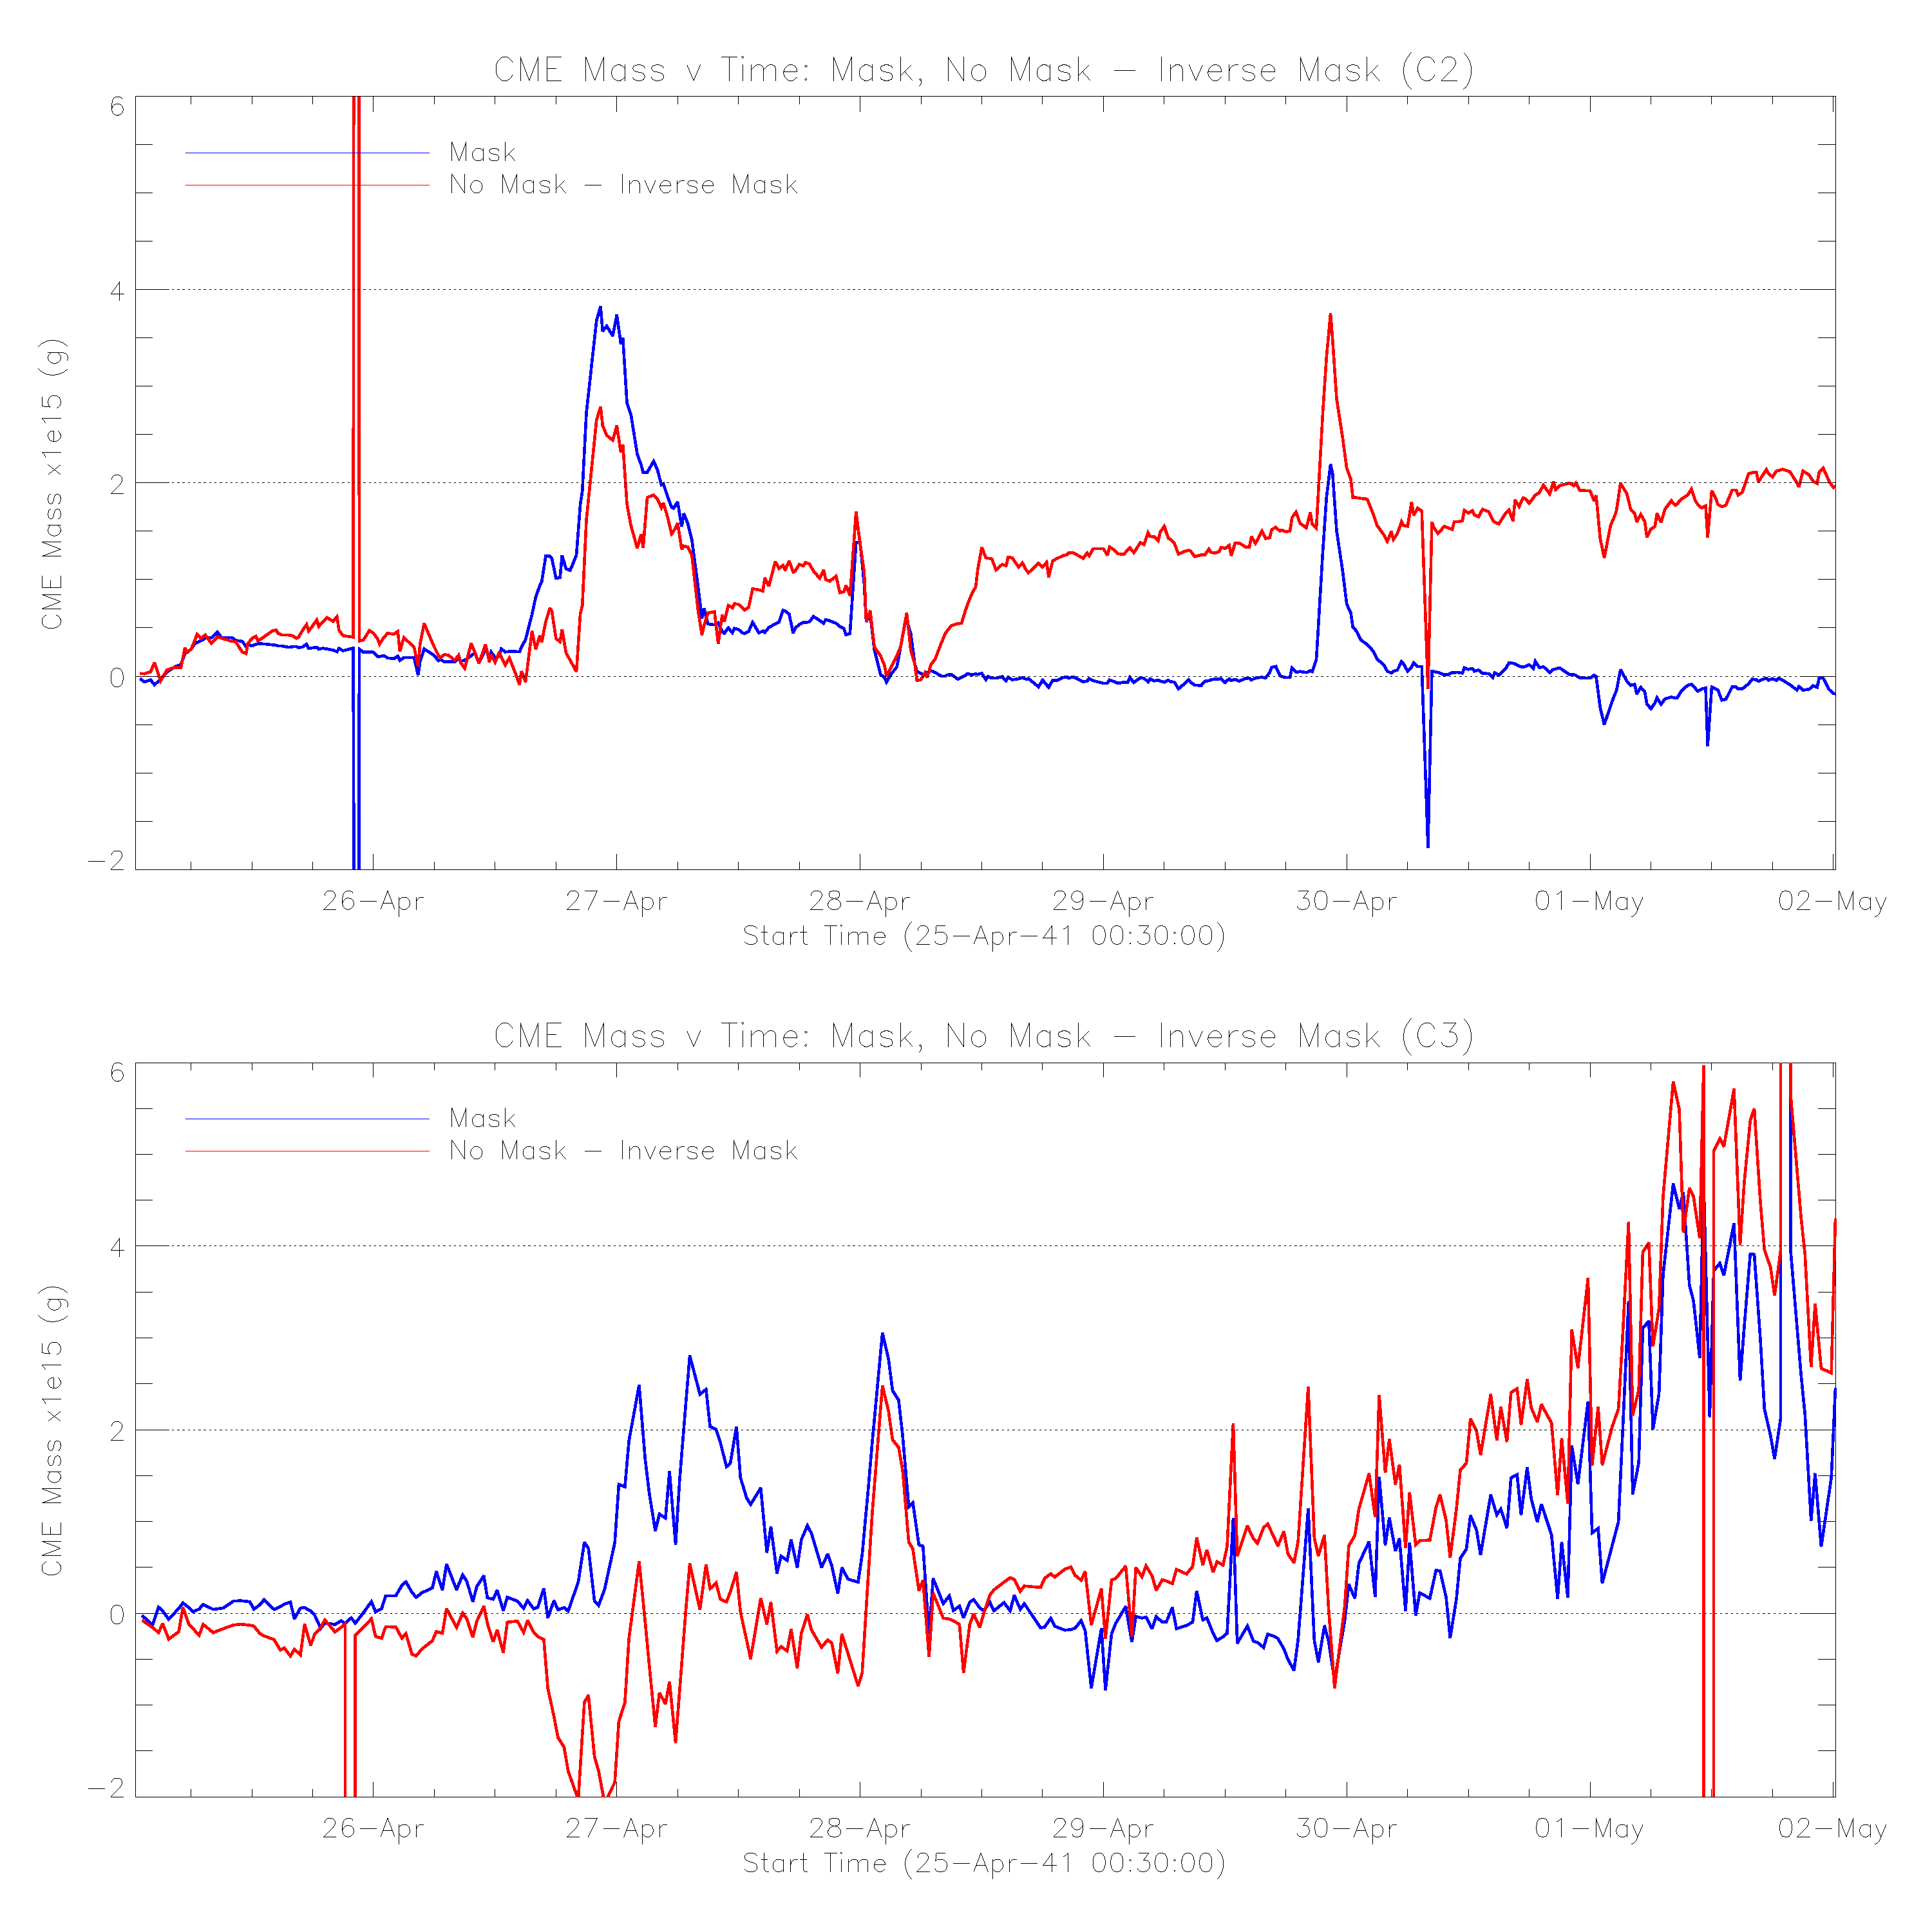
\includegraphics[scale=0.3]{mask_nomask_invmask_c2c3}
\caption{Comparison of the mass from masked images (blue) the no\_mask - inverse\_mask images (red) for C2 (upper) and C3 (lower). For both C2 and C3 the blue and red lines are a good match. The most obvious difference is the positive drift of the red line in C2, due to an excess background brightness subtracted in the base-differencing.}
\label{fig:comparison}
\end{center}
\end{figure}
The over-bright pre-event image used in the base difference is drawing the background values in no-mask and invert-mask into negative values. The blue line in Figure~\ref{fig:comparison0} (upper panel) should sit at zero, while the orange line should only show positive values when a CME is in the frame. The fact that they both drift into the negative means they will result in a positive excess when subtracting the two.
Algebraically, the procedure resulting in the red line in Figure~\ref{fig:comparison} is as follows:
\begin{equation}
y = \sum(I_{img} - I_{pre}) - \sum[(I_{img} - I_{pre})\times (1-I_{mask})]
\label{eqn:criteria_test}
\end{equation}
where $I_{img}$ is the current image and $I_{pre}$ is pre-event image; $I_{img} - I_{pre}$ represents a base difference. $(1-I_{mask})$ is the inverted mask. Ideally, Equation~\ref{eqn:criteria_test} would result in
\begin{equation}
y = M_{cme} - 0
\label{eqn:no_problem}
\end{equation}
However due to excess brightness in the pre-event image we end up with a negative mass value $M_{neg}$ combined with the CME mass $M_{cme}$
\begin{equation}
y = (M_{neg} + M_{cme})  - M_{neg}
\end{equation}
Since $M_{neg} < (M_{neg} + M_{cme}   ) < 0$, we end up with $y$ value that is positive and larger than $M_{cme}$. Of course, if the pre-event image were chosen appropriately we would just have Equation~\ref{eqn:no_problem}, no problem. It's interesting to note that the difference between the blue and red line in Figure~\ref{fig:comparison} is a measure of how much the background corona changed over time; it is also a measure of how well chosen the background image is for the base-difference. If the lines diverge consistently, too much background brightness has been extracted from the images. The effect is not as pronounced in C3 for the observation sequence, probably because the CME does not perturb the background corona at this height range as much as it does at lower heights (in C2 FOV). Hence the analysis resulting in Figure~\ref{fig:comparison} are a way of confirming that criteria (i) and (ii) are fulfilled.

There are a number of questions and issues that need to be addressed if the automatic mass detection is to produce reliable results:
\begin{itemize}
\item Removal of the spurious blobs in the quiet-time masks. Background values need to be brought to a maximum of $10^{13}$\,g, this will ensure detection of even small CMEs with masses of $\sim$$10^{14}$\,g.
\item An algorithm to choose an appropriate prevent image needs to be implemented. An average of a set of quiet images before CME detection is a possibility. 
\item What mass value should be taken as being representative of the CME mass? Is it appropriate to take the maximum mass value detected during the time interval when the CME is present? If so, should the maximum mass be taken from C2 or C3?
\end{itemize}
The last item here will require a a number of tests to be performed on which telescope can provide the most reliable mass estimate. Primarily, C3 would seem like the most appropriate, since the large field-of-view (FOV) can contain all CME material i.e., there will be some material hidden by the occulter, as can happen in the C2 FOV. However, C3 is more susceptible to POS errors e.g., if the CME is not actually on the POS, the uncertainties introduced by assuming it \emph{is} on the POS are worse for C3. 
%There main pros and cons of each coronagraph are
%\begin{itemize}
%\item C2 \hfill \\
%-Pro: CME is closer to POS \\
%-Con: Mass is hidden behind disk
%\item C3 \hfill \\
%-Pro: FOV is large enough to view all CME (smaller mass-hiding)\\ 
%-Con: Very bad POS effects
%\end{itemize}
These may be addressed by a study of the Thomson scattering geometry of the light received by each telescope.

%Finally, the inherent uncertainties on the CME mass a the most serious threat to the feasibility of automatic mass detection. Realistically, we can only give an order of magnitude estimate e.g., CME mass is somewhere between $10^{14}-10^{15}$\,g or $10^{15}-10^{16}$\,g etc. One idea is a CME mass classification into ranges such as
%\begin{itemize}
%\item A Mass: $10^{13}-10^{14}$\,g
%\item B Mass: $10^{14}-10^{15}$\,g
%\item C Mass: $10^{15}-10^{16}$\,g
%\item C+ Mass: $>10^{16}$\,g (on the off chance that mass is slightly above C)
%\end{itemize}
%With such a system you could say there was a \textquoteleft C' mass CME on such a date and time, without having to quote some uncertain mass estimate. The uncertainties might result in the mass transcending two classes, in that case you could then quote \textquoteleft BC' mass. In practice, such large ranges may be the only way in which CME mass values can be presented in a catalogue. Despite such limitations, this may be useful to any user wishing to search for events that have small, intermediate, or large energies.

\subsubsection{Mass Estimates with AIA}
\begin{figure}[t!]
\begin{center}
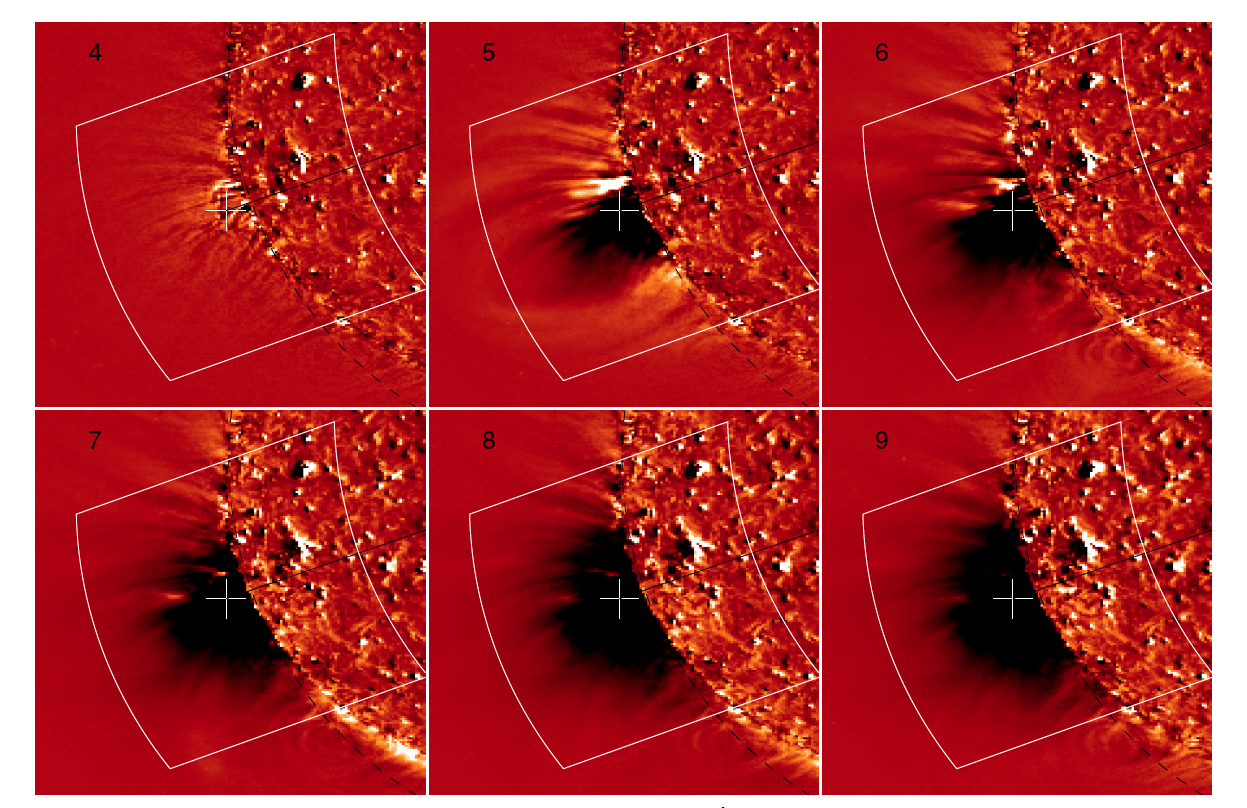
\includegraphics[scale=0.35, trim=1cm 0cm 0cm 1cm]{euv_dimming.png}
\caption[EUVI dimming region]{EUV dimming region observed by EUVI 195\,\AA~channel on 31 December 2007. The dimming is due to evacuation of plasma from the region such that the emission measure drops \citep{aschw09}}
\end{center}
\end{figure}
There a number of studies that have determined the mass of CMEs with varying degrees of accuracy from white-light observations. However very few studies, if any, have investigated where exactly the CME mass comes from. The origin of the mass is difficult to determine since the very early stages of CME development are obscured by the occulting disk of a coronagraph. This means that EUV imagers of the low corona are currently the only viable method of observing the birth of a CME. An analysis of the mass development during such an early phase of eruption may be able to reveal both the origin of the mass and what ultimately forms the CME. Currently, these are two major unknowns in CME physics.

The eruption of a CME in EUV observations is usually conspicuous by a lack of emission in the erupted active region i.e., as the CME erupts it evacuates the corona, leaving behind an emission deficit. This emission deficit is known as an EUV `dimming' region and has been used to calculate the amount of evacuated mass \citep{aschw09}. Dimming regions are also a regular feature of soft X-ray images \citep{sterling1997}.
%
%
%
\begin{figure}[t!]
\begin{center}
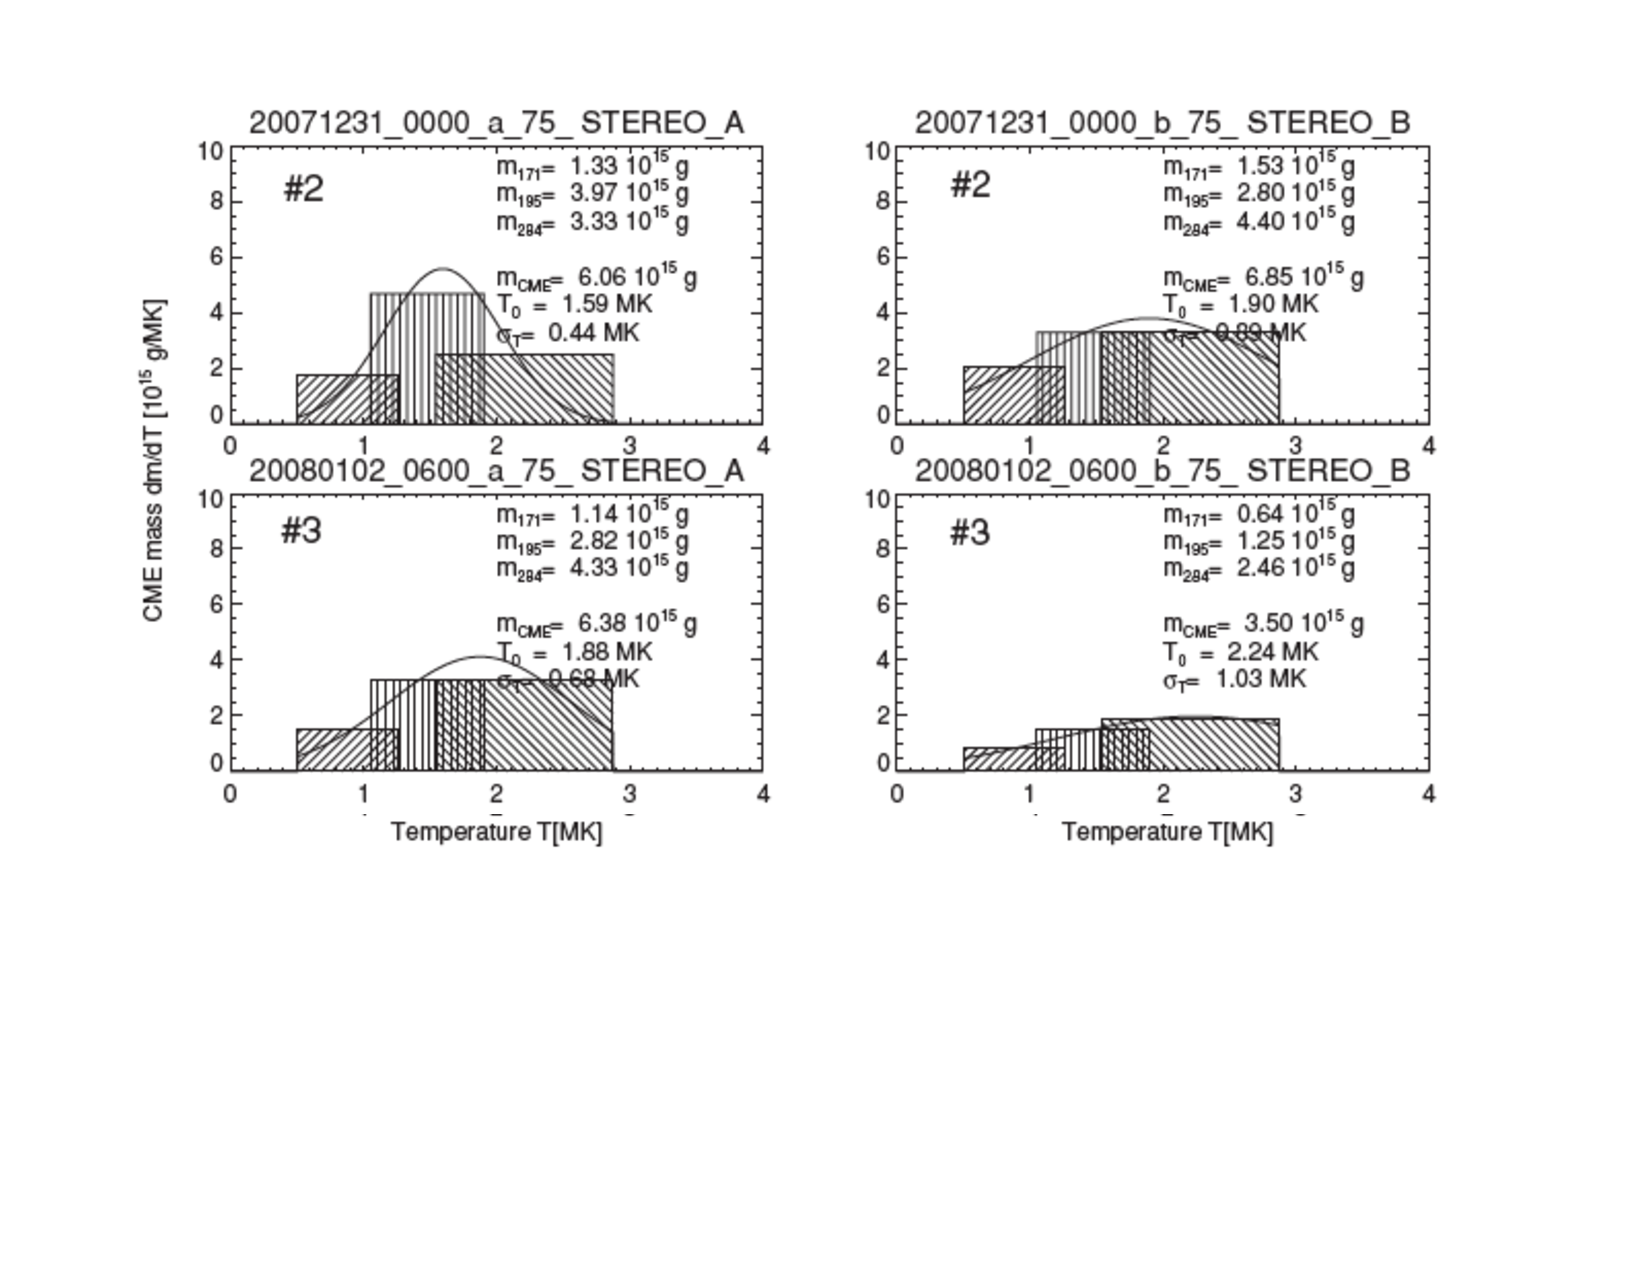
\includegraphics[scale=0.56, trim=1cm 7cm 0cm 2cm]{mass_temp_dist2.pdf}
\caption[Mass-temperature distribution]{Mass-temperature distribution from EUVI/A and B for five different events. The three channels if EUVI, 171\,\AA, 195\,\AA, and 284\,\AA, are used to calculated the mass of the material contributing to emission in each of these channels. A construction of a Gaussian using these three measurements allows integration over temperature to find the total CME mass in the temperature range of 0.5--3.0\,MK. Adapted from \citep{aschw09}}
\label{fig:euvi_mass}
\end{center}
\end{figure}


The method of \citet{aschw09} exploits the fact that there are multiple filters in EUV imagers that can be used to measure the amount of evacuated mass in dimming regions. In one filter, the evacuated mass, $m_d$, may be calculated from
\begin{equation}
m_d(t,T) = m_p n_d(t)V_D = m_p n_A\sqrt{\frac{I_d(t)}{I_A}}\frac{\pi}{4}w_d^2\lambda_T
\end{equation}
where $m_p$ is proton mass, $n_d$ is dimming number density, $V_D$ is dimming volume, $n_A$ is active region density (pre eruption), $I_d$ is dimming region intensity, $I_A$ is active region intensity (pre-eruption), $w_D$ is the radius of the circular footprint of the dimming region, and $\lambda_T$ is the temperature scale height. Since $m_d$ may be measured in each of the temperature filters of the EUV imager the total mass may be constructed from a differential emission measure-type mass distribution
\begin{equation}
m_{cme}(t)=\int_{T_1}^{T_2}\bigg( \frac{dm_d(t,T)}{dT} \bigg)dT = \int_{T_1}^{T_2}\frac{\Delta m_D}{\Delta T_F}\mathrm{exp}\bigg( -\frac{(T-T_0)^2}{2\sigma_T^2} \bigg)dT
\label{eqn:tot_euv_mass}
\end{equation}
This analysis has been performed for EUVI on STEREO A and B. This imager only has three different passbands at 171\,\AA, 195\,\AA, and 284\,\AA, representing only three data points to which a gaussian is fit to the mass temperature distribution in Equation~\ref{eqn:tot_euv_mass}, these fits are shown in Figure~\ref{fig:euvi_mass}.
Since this may be done over time for each EUV image in the observation sequence, \citet{aschw09} constructed a mass evacuation curve over time (Figure~\ref{fig:mass_dim_time}). The curves correspond to different flares. This kind of analysis has the ability to give information on the eruption rate of the CME and possibly the forces acting on the ejection. However, not much work has been done in this area and the field is relatively under-explored. A number of interesting questions need to be investigated for for mass evacuation rates:
\begin{itemize}
\item Does mass evacuation rate depend on flare size?
\item Does evacuation rate depend on flare rise-time?
\item Is there any correlation with CME kinematical profiles?
\item Are the mass evacuation rate and final mass correlated?
\item Are mass evacuations different for events that have no associated flare?
\item Ultimately, why are some evacuation rates faster than others?
\end{itemize}
These questions need to be investigated if there is to be an advance in understanding the origins of CMEs. However, EUVI observations are limited in this regard.
\begin{figure}[t!]
\begin{center}
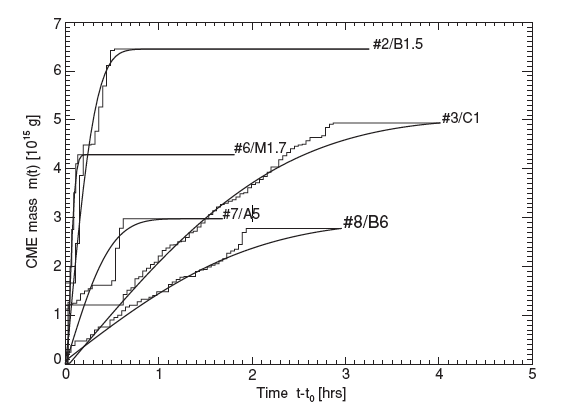
\includegraphics[scale=0.55, trim=1cm 0cm 0cm 1cm]{mass_dim_t.png}
\caption[Mass evacuation with time]{Mass evacuation from the dimming region with respect for five selected events. The biggest flare has the fastest mass loss rate but not the biggest final mass. \citep{aschw09}}
\label{fig:mass_dim_time}
\end{center}
\end{figure}
Since there is only three data points to which the Gaussian is fit to this mass-temperature distribution, the results are quite unconstrained and sometimes unreliable. For example, panels \#3 \emph{STEREO} B of Figure~\ref{fig:euvi_mass} is a bad representation of a Gaussian. This may be due to the CME plasma temperature lying outside the response of the three EUVI channels. Also, the cadence of EUVI may be too slow to capture the very early stages of mass evacuation, which would be needed if a comparison was to be made with an impulsive flare.

The possibility for advancing this kind of study with AIA is very promising. There are at least three main areas in which AIA can advance such research
\begin{itemize}
\item AIA has a possible six passbands that may be used in the mass distribution curve. This will enable a better constraint on the Gaussian in Equation~\ref{eqn:tot_euv_mass}, producing a more reliable total mass estimate than the three passbands of EUVI. Another result that may stem from this is investigating the temperature distribution of CME material, leading to a development in an understanding of CME thermal energies, which are often overlooked.
\item The above results could be advanced with the inclusion of UVCS spectroscopy data, which can give CME thermal characteristics from O\,VI, V and C\,III lines out to a height of $4\,R_{\odot}$. A comparison of early and intermediate phase CME temperatures could determine if the CME expands adiabatically, which is another unknown. This is important for investigating how isolated the CME is from the solar wind plasma.
\item AIA has a 12 second cadence (EUVI has 10 minutes), enabling a calculation of a mass evacuation curve in the very early stages of CME eruption. As mentioned, this will be particularly important for a comparison with very impulsive flares.
\end{itemize}
There are a wealth of physical properties in the early phase of CME eruption that could be answered with AIA. Up until current time, such an analysis has gone relatively unexplored.

\section{Coronal Shocks and Radio Bursts}

\subsection{Principle results}
The second goal of this thesis was to increase the understanding of CME-driven shocks and investigate the relationship amongst the various shock observables. A combination of white-light, EUV, and radio imaging showed CBFs and radio bursts have a common origin in a shock, and that this shock was driven by the CME flank. The principle results of this investigation were
\begin{itemize}
\item CBFs are closely associated to particle acceleration radio activity. The temporal correlation between CBFs and radio bursts such as type IIs and type IIIs has been highlighted in the past \citep{klassen2000, maia2004}. However, there are very few, if any, direct observations of an association between radio sources and CBFs. \citet{vrsnak2005a} showed a radio source which propagated around the limb in association with a CBF, however any direct comparison between the two features was hampered by the low cadence of EUV imaging. To date, the Carley {\emph et al.} (2013) observation of a 150\,MHz source closely following a CBF is the most comprehensive presentation of the clear relationship between the two features (Figure~\ref{fig:figure_aia_nrh_c2}). It has confirmed that CBFs are inherently associated with radio activity. This radio activity is plasma emission generated by an instability in the presence of electron beams.
\item The kinematics of the radio source was analysed giving a measure of the speed of this source. In order to estimate its Alfv\'{e}n Mach number, we performed density and magnetic field diagnostics of the corona. Density diagnostics were taken from six AIA passbands and LASCO C2, while the magnetic field measurements were performed using a PFSS extrapolation. The combined density and magnetic field maps allowed us to produce an Alfv\'{e}n speed map of the corona (Zucca {\emph et al.} (in prep)). To our knowledge, this was the first time such a map was produced from observations. It provided a reliable means of comparing the source speed to the Alfv\'{e}n speed of the corona in order to estimate the source Alfv\'{e}n Mach number.
\item The density map was also used in the analysis of the radio bursts in the dynamic spectra of S/WAVES, Nan\c{c}ay DA, and RSTO eCallisto. Usually, density models are employed to derive particle kinematics from drift rates in dynamic spectra. However, this can lead to erroneous positions and speeds of the particles producing the radio emission because the density models may be an unreliable description of coronal density profiles. Use of the density diagnostics from observation allowed us to derive much more reliable coronal heights for the radio activity observed in the dynamic spectra
\item Analysis of the dynamic spectra activity showed there was particle acceleration of up to 0.4\,$c$, which manifests in the spectra as type III radio bursts. The speed of these bursts along the parker spiral were used to estimate an ETA of the electrons at the STEREO -B spacecraft. It was found the ETA matched the observed time of arrival quite accurately. Furthermore, the observations of herringbones were the most striking evidence for particle acceleration in this study. The observations of herringbone fine structure were made possible by the installation of RSTO eCallisto spectrometers, as described in Chapter 3. The dynamic spectra from RSTO produced some of the clearest spectra of these herringbone bursts during the 22 September 2011 event, compared to other dynamic spectra observations. An analysis of these bursts showed that they are produced by electrons at a speed of 0.15\,$c$ and occur with a quasiperiodicity of 2-11 seconds.
\item Both the radio source imaged by NRH and CBF had a close association with the southern flank of the CME. Since the a thermal analysis of the CBF showed that it was most likely a pressure wave, and the radio source was associated with spectral shock activity, we conclude that a shock driven by the CME flank expansion was the likely driver of CBF and radio activity. Evidence for a shock at the CME flank also came in the form of white-light observations. These observations were used to reconstruct the CME in 3D dimensions and show that the faint feature observed to the south of the CME in LASCO C2 was not part of the CME structure, and therefore must be shock.
\end{itemize}
Overall, this work has shown how a combination of radio, EUV and white-light imaging can reveal the evolution of plasmoid driven shocks in the solar atmosphere. It has shown that CBFs and radio bursts can share a common origin in a shock driven by the expansion of a CME flank.

\subsection{Future Work}

\subsubsection{Hough Transform and Herringbone Statistics}
\begin{figure}[t!]
\begin{center}
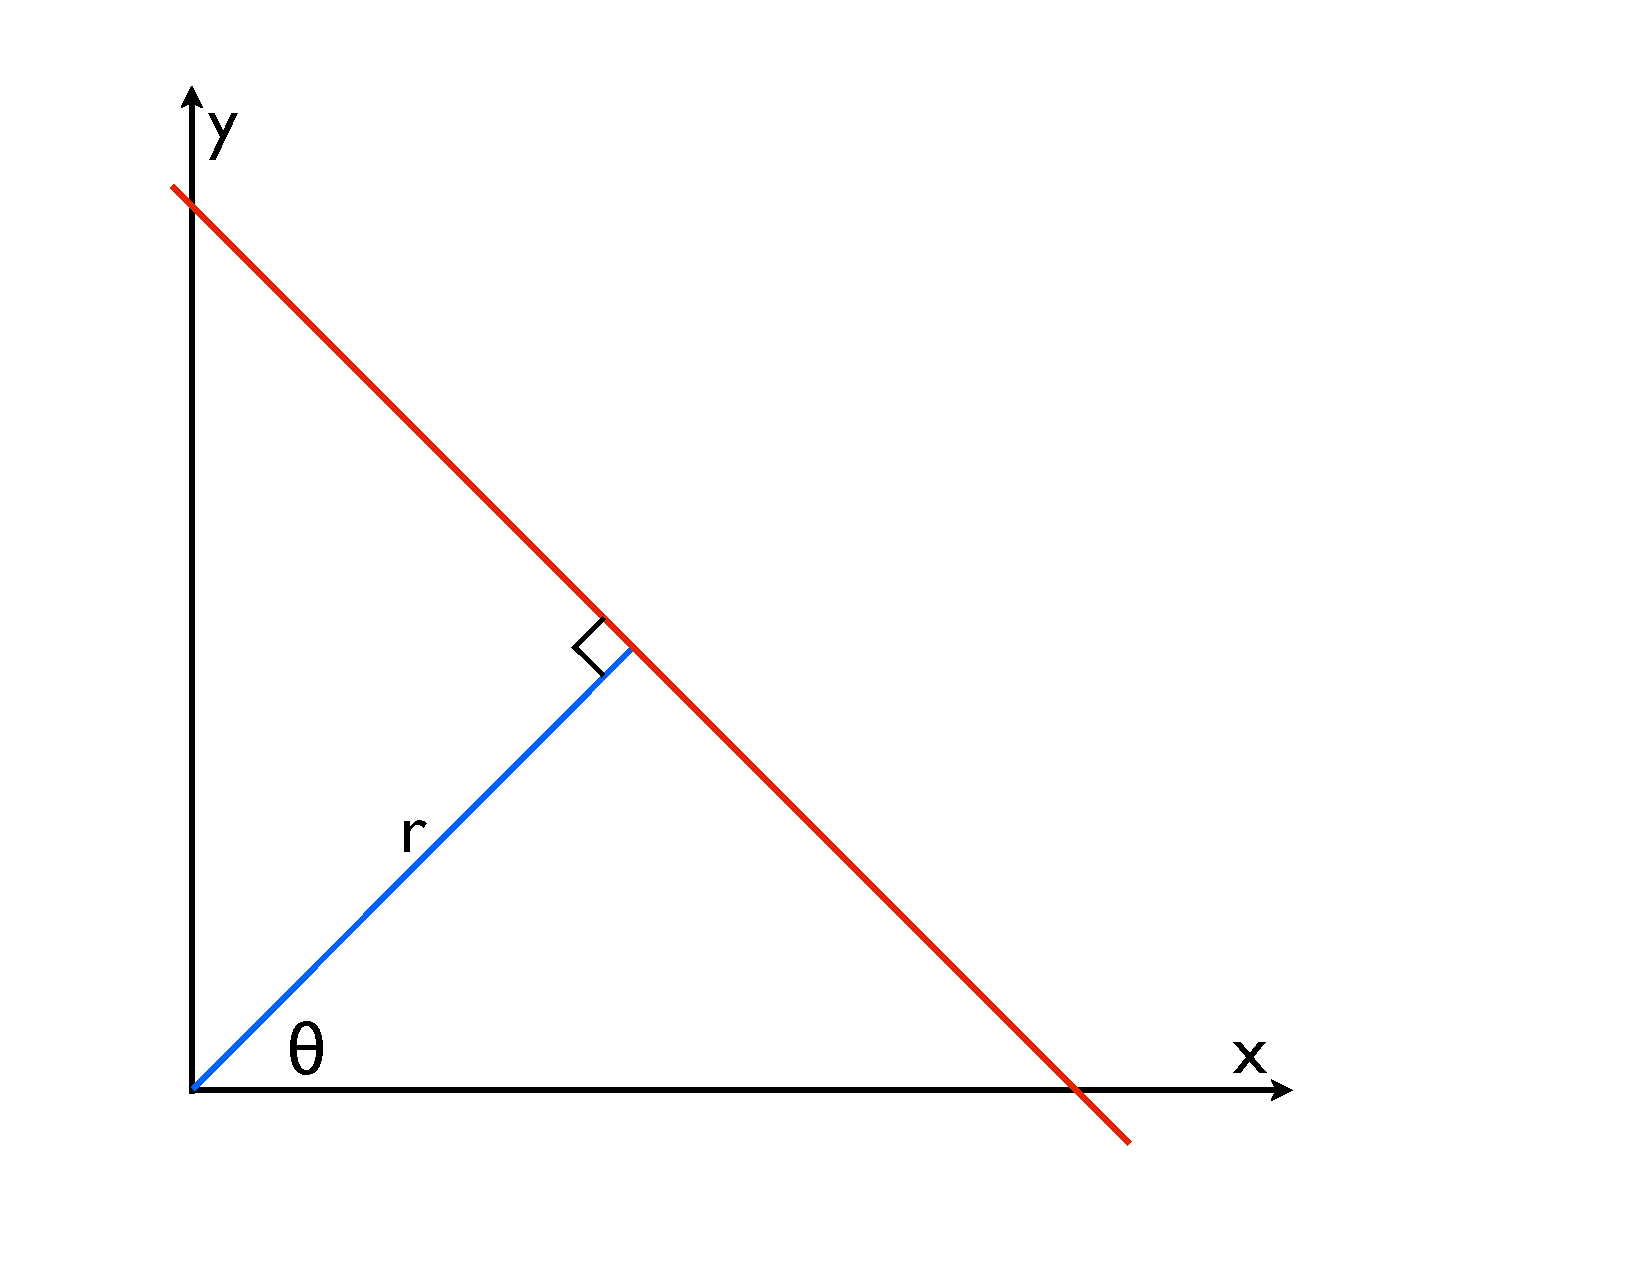
\includegraphics[scale=0.4, trim=0cm 2cm 3cm 1.5cm]{r_theta_line.pdf}
\caption[Line in polar coordinates]{Line in the image space $(x,y)$ and its polar coordinates $(r, \theta)$. These two sets of coordinates are used to form a relationship by the image space and an $(r, \theta)$ Hough parameter space. For any orientation of the line through $P$ (red line) the vector $r$ (blue line) must intersect it at right angles. Rotating the red line about $P$ will give a range of $(r, \theta)$ values that represent all red line orientations passing through $P$. These $(r, \theta)$ values will form a sinusoid when plotted in an $(r, \theta)$ space.}
\label{fig:r_theta_line}
\end{center}
\end{figure}
As mentioned in Chapter 5, the frequency drift of herringbones can give information on the particle speeds, whereas there behaviour over time may depend on the shock acceleration characteristics. Also, the emissivity of plasma emission depends on the velocity of the particles inducing the emission (Equation~\ref{eqn:plasma_emiss}). However, it is still unknown as to what causes the herringbone bursts. Since there are many bursts in one herringbone sequence, there is an opportunity to statistically investigate the drift rates and intensities of these bursts, which can reveal details of the particle acceleration process, and the plasma emission process.

To perform this statistical analysis we use the Hough transform \citep{hough1961}, a feature recognition algorithm that is used to identify straight lines in images \citep{duda1972}. In the Hough transform any line in an image may be represented in polar coordinates as $r=x\mathrm{cos}\theta +y\mathrm{sin}\theta$ (Figure~\ref{fig:r_theta_line}). Any point $P$ in the images space at $(x_0, y_0)$ will have many lines, described by $(r,\theta)$, that pass through it. In fact, all the values of $(r, \theta)$ which represent lines passing through $(x_0, y_0)$ will form a sinusoid in an $(r,\theta)$ parameter space known as Hough space. The relationship between the images space and Hough space is shown in Figure~\ref{fig:image_hough}. The sinusoid in Hough space is unique to the point $(x_0, y_0)$. Now, a second point in the image space, $(x_1, y_1)$, will also have its own unique sinusoid in Hough space. The point $(r_i,\theta_i)$ at which these sinusoids intersect represents a line that passes through both points in the image space, given by
\begin{equation}
y = \bigg(- \frac{\mathrm{cos_i}\theta}{\mathrm{sin}\theta_i}\bigg)x + \bigg(\frac{r_i}{\mathrm{sin}\theta_i}\bigg)
\end{equation}
\begin{figure}[t!]
\begin{center}
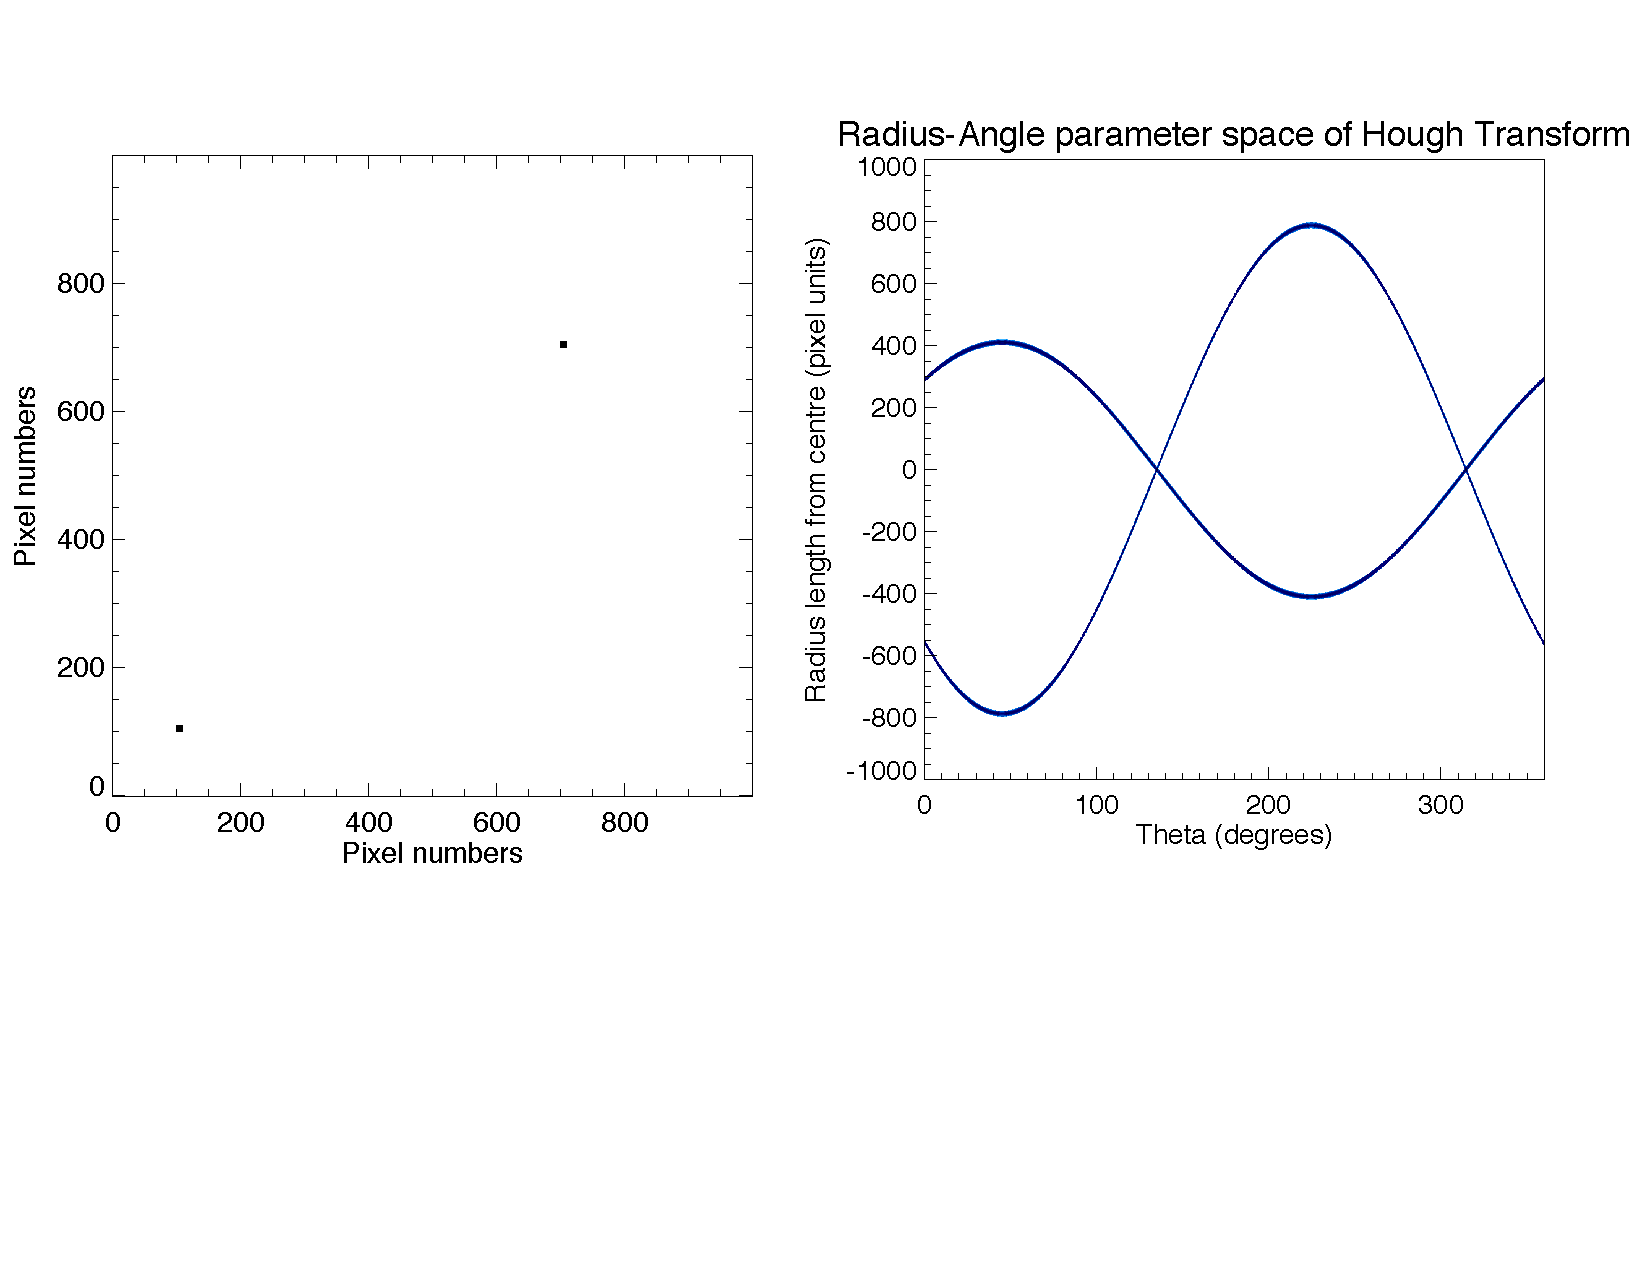
\includegraphics[scale=0.5, trim=0cm 6cm 0cm 1.5cm]{hough_example_simple}
\caption[Relationship between image space and Hough space]{Relationship between image space and Hough space. The point in the image space have a range of $(r, \theta)$ points which represent all lines passing through the point. The $(r,\theta)$ values are sinusoids for each point, their point of intersection in Hough space will give the $(r_i, \theta_i)$ of the line passing through the points int he image space.}
\label{fig:image_hough}
\end{center}
\end{figure}
If a number of points in an image lie along a straight line, each of these points will have its own sinusoid in the Hough space and the point at which these sinusoids intersect represents the line that passes through all of the image points. A `back-projection' of this Hough space to image space then returns the original image. Two examples if this are given in Figure~\ref{fig:hough_example}. The top row shows an image of a number of lines of varying orientation and a square. The middle panel shows the $360^{\circ}$ Hough space. Note that the sinusoids intersect at $90^{\circ}$ (horizontal line), $180^{\circ}$ (vertical line), and $135^{\circ}$ diagonal line. 
\begin{sidewaysfigure}
\centering
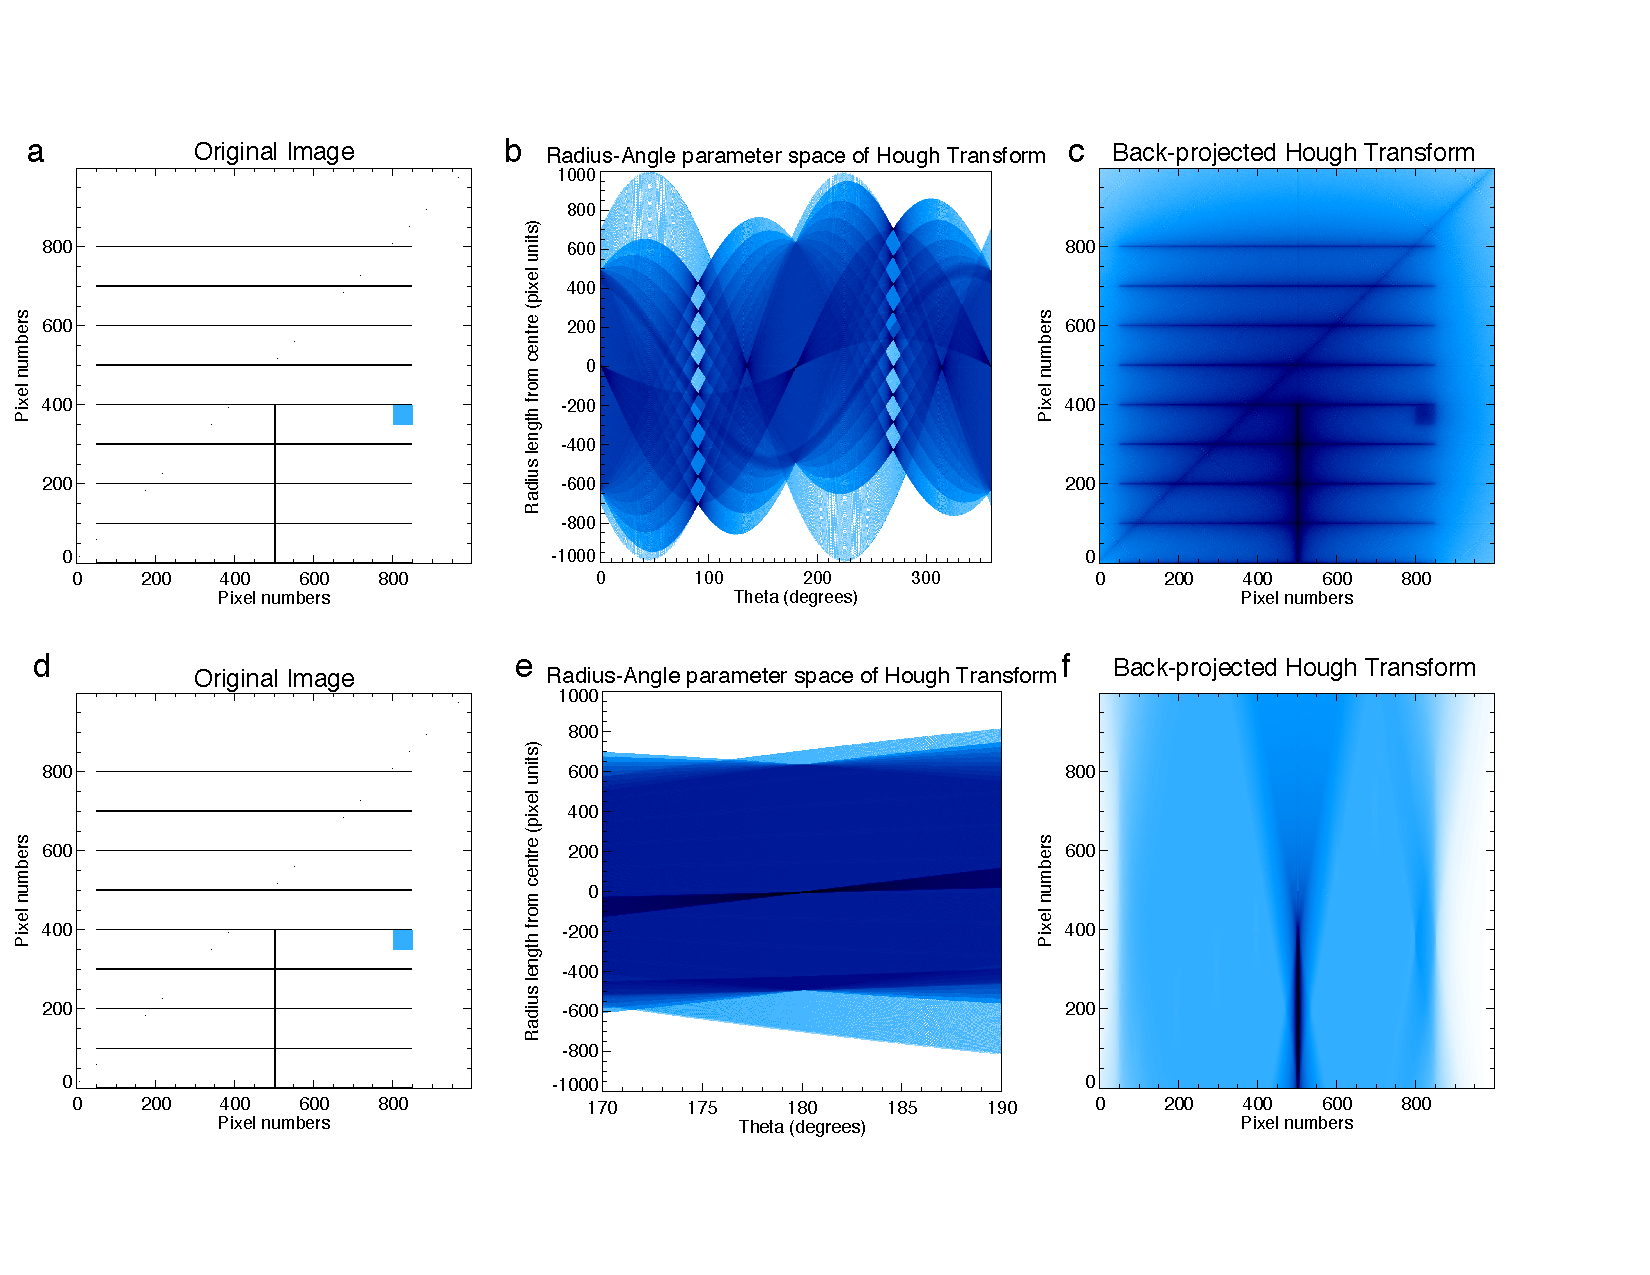
\includegraphics[scale=0.7, trim=0cm 2.5cm 2cm 1.5cm]{hough_example.pdf}
\caption[Example Hough Transform]{(a) An image with a number of lines of varying orientation and intensity. (b) The Hough transform of the image in $(r, \theta)$ space. The multiple intersection points at $90^{\circ}$ and a variety of radii correspond to the multiple horizontal lines in the original image. There are also intersection points at $135^{\circ}$ (diagonal line in original image) and $180^{\circ}$ (vertical) line. (c) The back projected Hough transform, recovering all features in the original image. The bottom row (d)-(f) show the same as the top row, expect that the back-projection is chosen over a region in hough space that only contains the vertical line. In this way only the vertical line is recovered and the remaining features are not recovered.}
\label{fig:hough_example}
\end{sidewaysfigure}
The square represents a whole variety of sinusoids in the hough space that intersect at all angles, this is because there are a range of lines that represent this filled square. Back-projection of the whole $360^{\circ}$ space returns all lines in the original image. However, we may only back-project the Hough space in a particular angular range to extract lines of a desired orientation. This is shown in the bottom row of Figure~\ref{fig:hough_example}. For the same original image we may isolate the vertical line, by only back-projecting the range $170^{\circ}-190^{\circ}$. Note the sinusoid intersection at $180^{\circ}$ (vertical line) in the `zoomed' Hough space (panel e). The back-projection shown in Figure~\ref{fig:hough_example}f contains the vertical line, and the vertical sections of the square.
%

\begin{figure}[t!]
\begin{center}
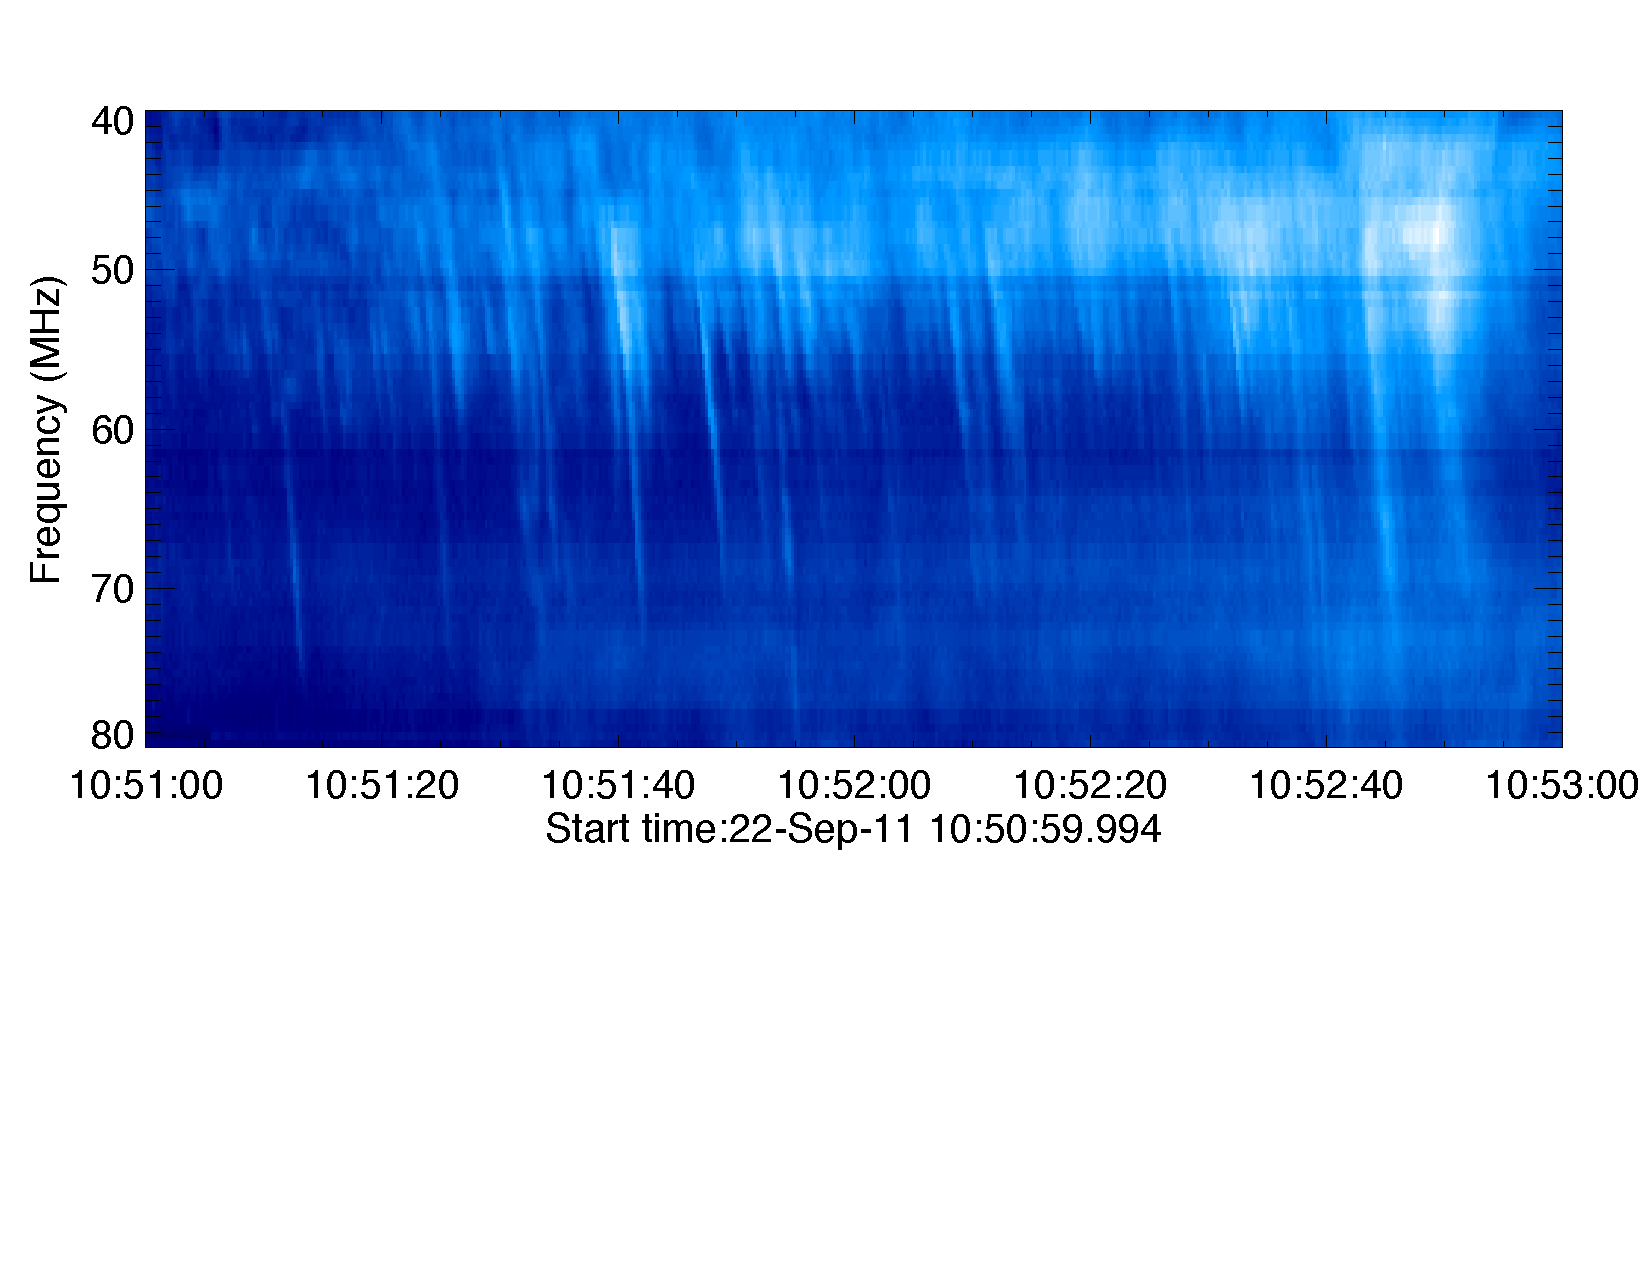
\includegraphics[scale=0.5, trim=0cm 7cm 0cm 2cm]{herringbones_only.pdf}
\caption[Herringbone observations]{The herringbone observations from RSTO eCallisto on 22 September 2011. Given the polar coordinates defined in Figure~\ref{fig:r_theta_line}. The herringbone orientations have an angle of $\sim$180--190$^{\circ}$.}
\label{fig:herringbones_only}
\end{center}
\end{figure}
Since the herringbones represent a large number of straight lines in a dynamic spectrum, a number of tests were performed with the Hough transform to investigate it's use as a feature detection algorithm for these bursts. The Hough transform was performed on an RSTO eCallisto dynamic spectrum of herringbone radio bursts shown in Figure~\ref{fig:herringbones_only}. The $360^{\circ}$ parameter space of the Hough transform is shown in Figure~\ref{fig:hough_space}. The overwhelming majority of detections are at an angle of $90^{\circ}$ corresponding to horizontal lines. This is most likely caused by RFI in the dynamic spectrum. Interpolation amongst frequency channels in the spectrum can also cause broad horizontal lines, this is particularly apparent in Figure~\ref{fig:herringbones_only}.
\begin{figure}[t!]
\begin{center}
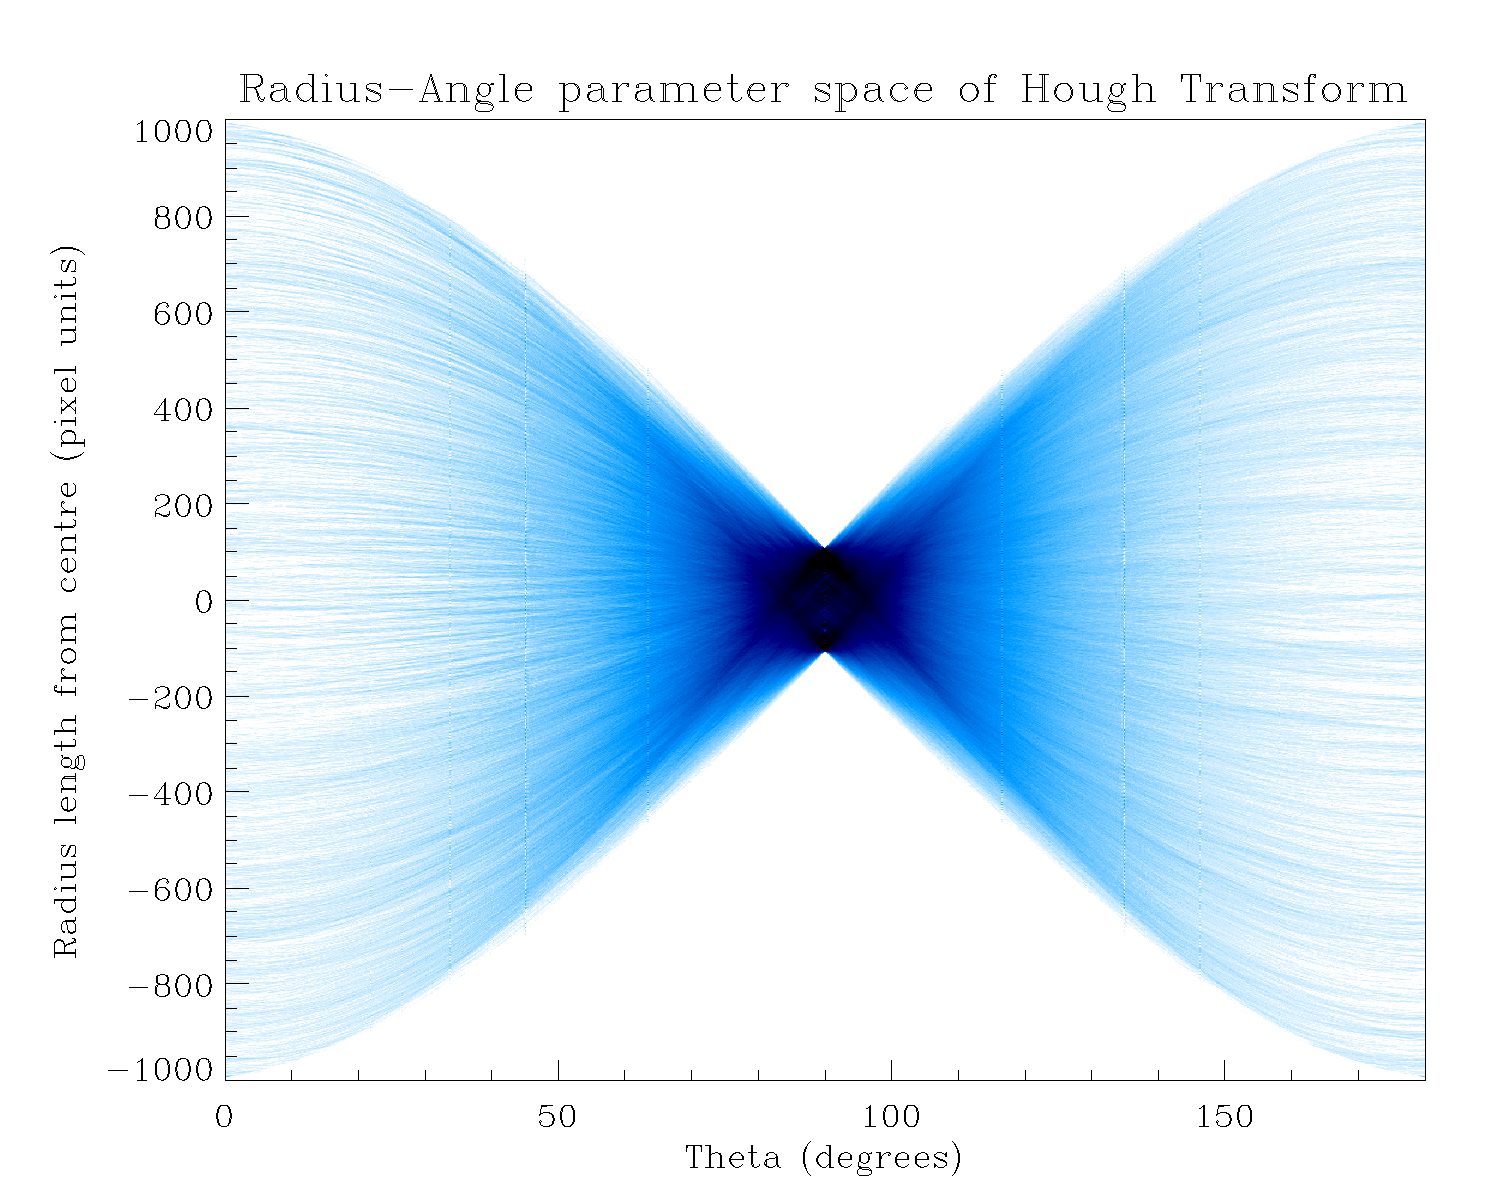
\includegraphics[scale=0.5, trim=0cm 1cm 0cm 1cm]{hough_herringbones}
\caption[Hough transform]{The radius-angle parameter space of the hough transform for the herringbones. The overwhelming majority of detections are at an angle of $90^{\circ}$ corresponding to horizontal lines, most likely caused by RFI and interpolation between frequency channels.}
\label{fig:hough_space}
\end{center}
\end{figure}
%
%

Despite the fact there are strong detections for horizontal lines, the multiple threads in the parameter space cross each other at all angles, which means lines of every orientation are detected. An {\it a priori} choice of angles in the parameter space that the herringbones belong to will allow them to be detected effectively. A range of angles of $180^{\circ}-190^{\circ}$ was chosen for the back-projection, the results of which are shown in Figure~\ref{fig:hough_hb}. Th transform was succesful in pcking out many of the herringbones, but missed the particularly weak ones. Although the transform is successful in picking out straight lines, it contains no information on the start and end point of the line. This is the reason why some bursts have a long length in the Hough transform detections, but a short length in the original dynamic spectrum. This mismatch of burst lengths is not a concern since the start and stop frequencies are not under investigation here. The identification of points that the bursts belong to allowed a number of parameters to be analysed and compared for each burst.
%
%
\begin{figure}[t!]
\begin{center}
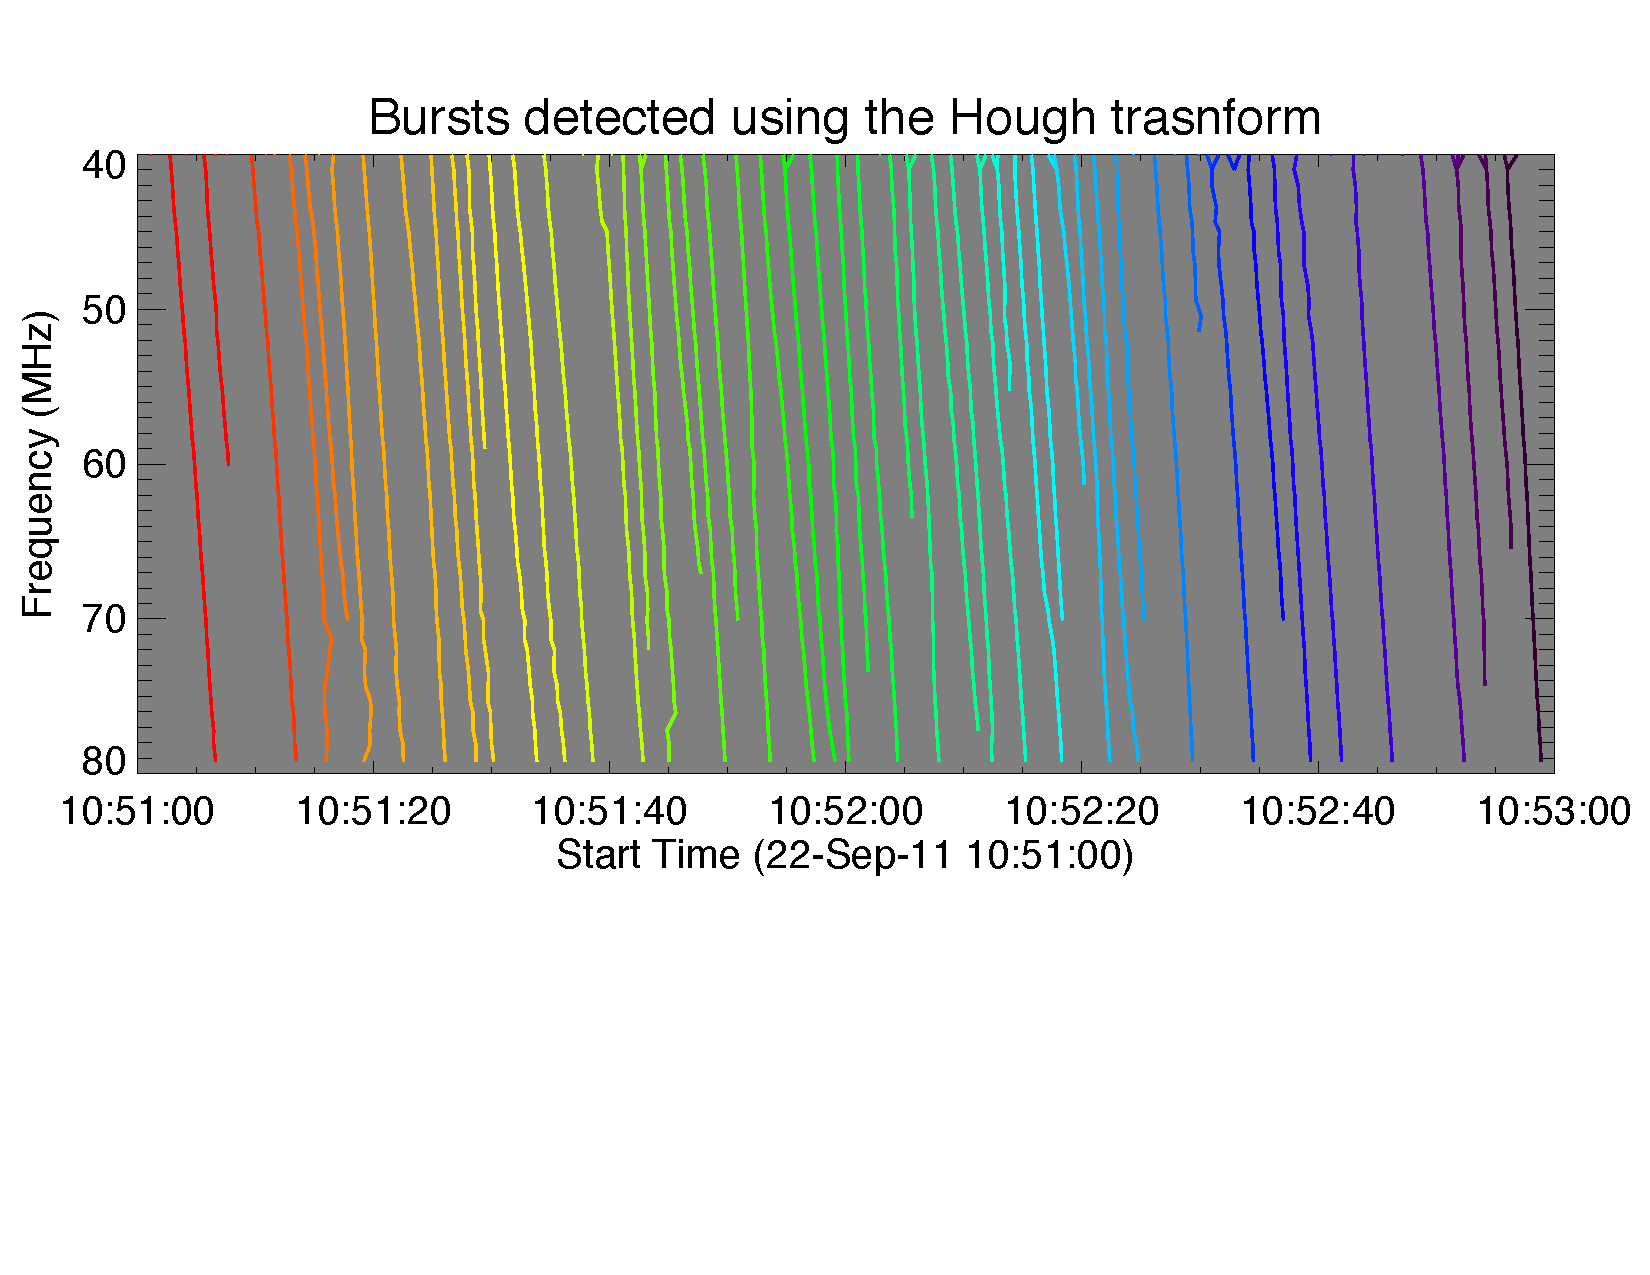
\includegraphics[scale=0.5, trim=0cm 7cm 0cm 2cm]{hough_herringbones_only}
\caption[Hough transform herringbones]{Herringbone bursts detected using the Hough transform. The Hough transform was successful in detecting most of the herringbones but failed to detect the weaker ones. The colours correspond to the statistical results shown below.}
\label{fig:hough_hb}
\end{center}
\end{figure}
%
%
\begin{figure}[t!]
\begin{center}
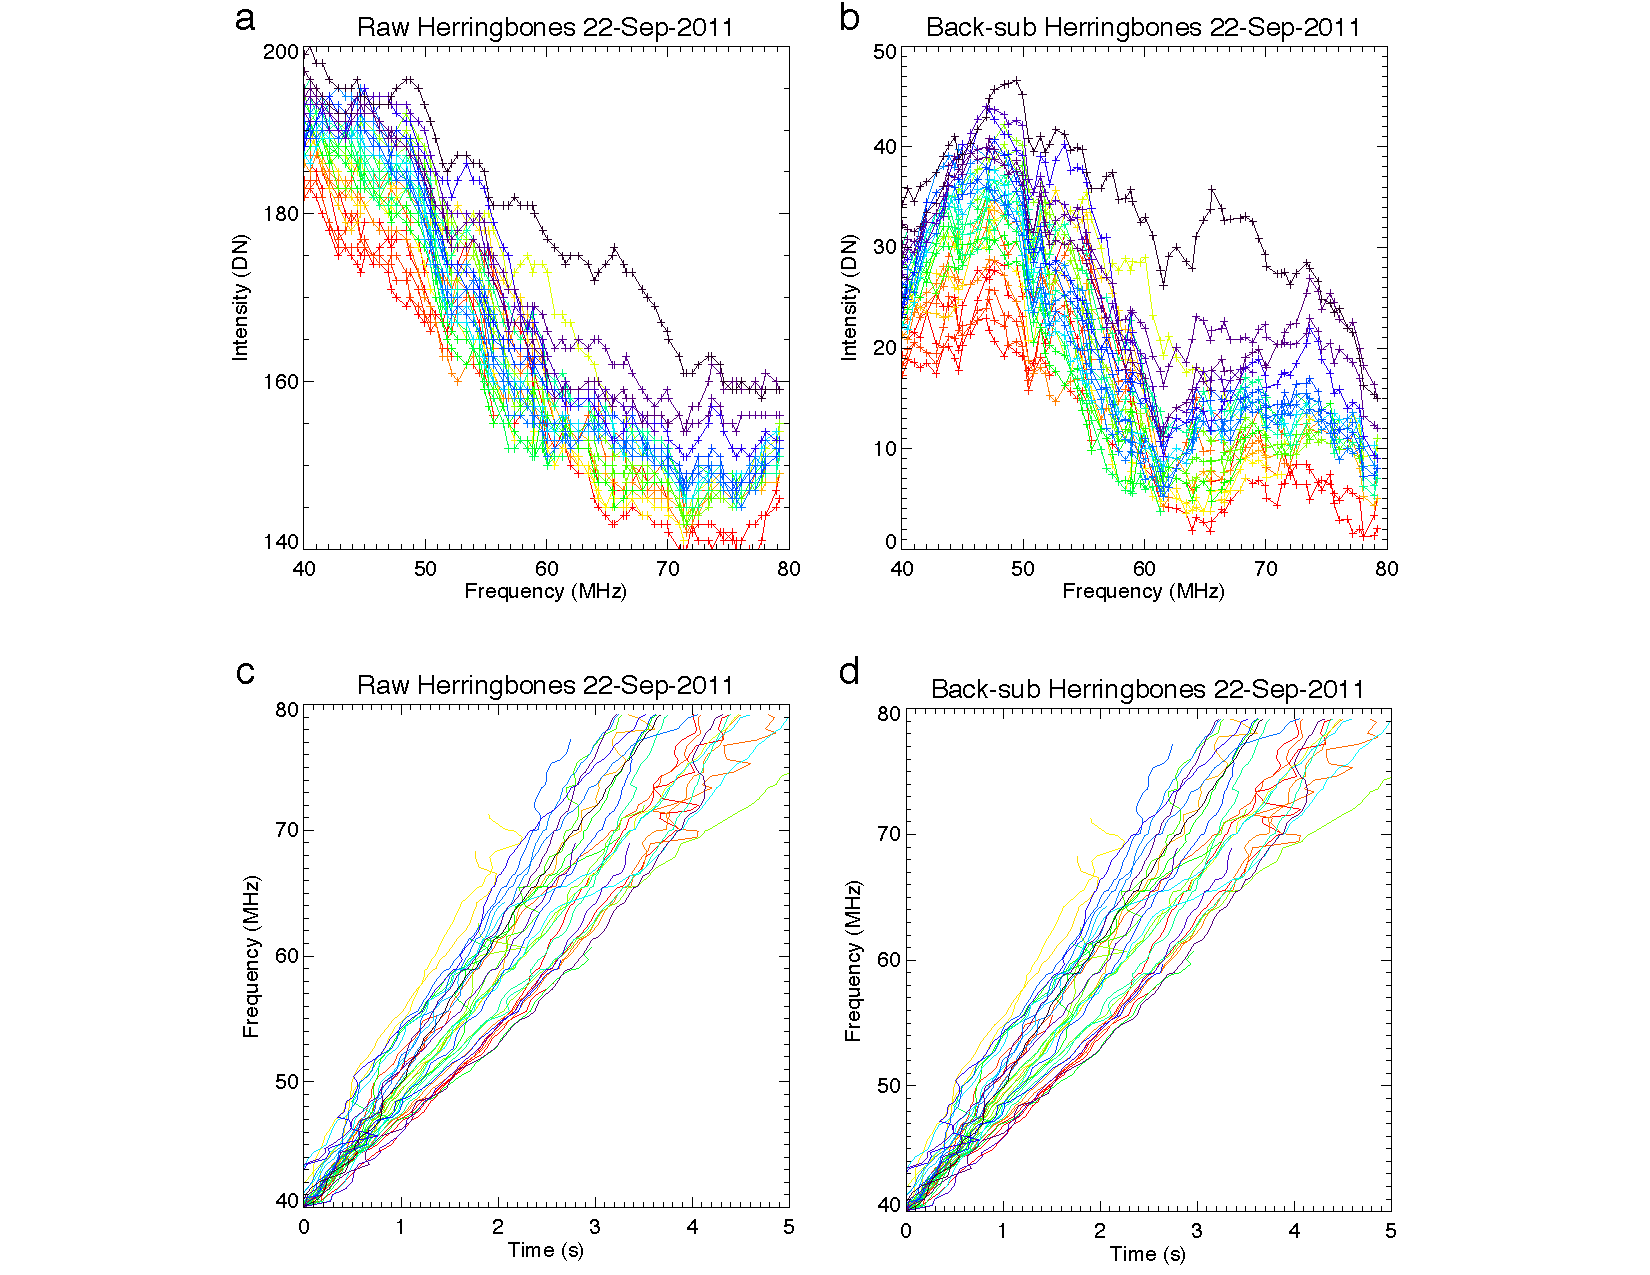
\includegraphics[scale=0.7, trim=3.5cm 0cm 0cm 1cm]{herringbone_stats.pdf}
\caption[Hough transform herringbones]{Herringbone bursts detected using the Hough transform. The transform performs well when the bursts are intense, but performs poorly when they are weak and close to background values.}
\label{fig:bibf}
\end{center}
\end{figure}


%
%
\begin{figure}[t!]
\begin{center}
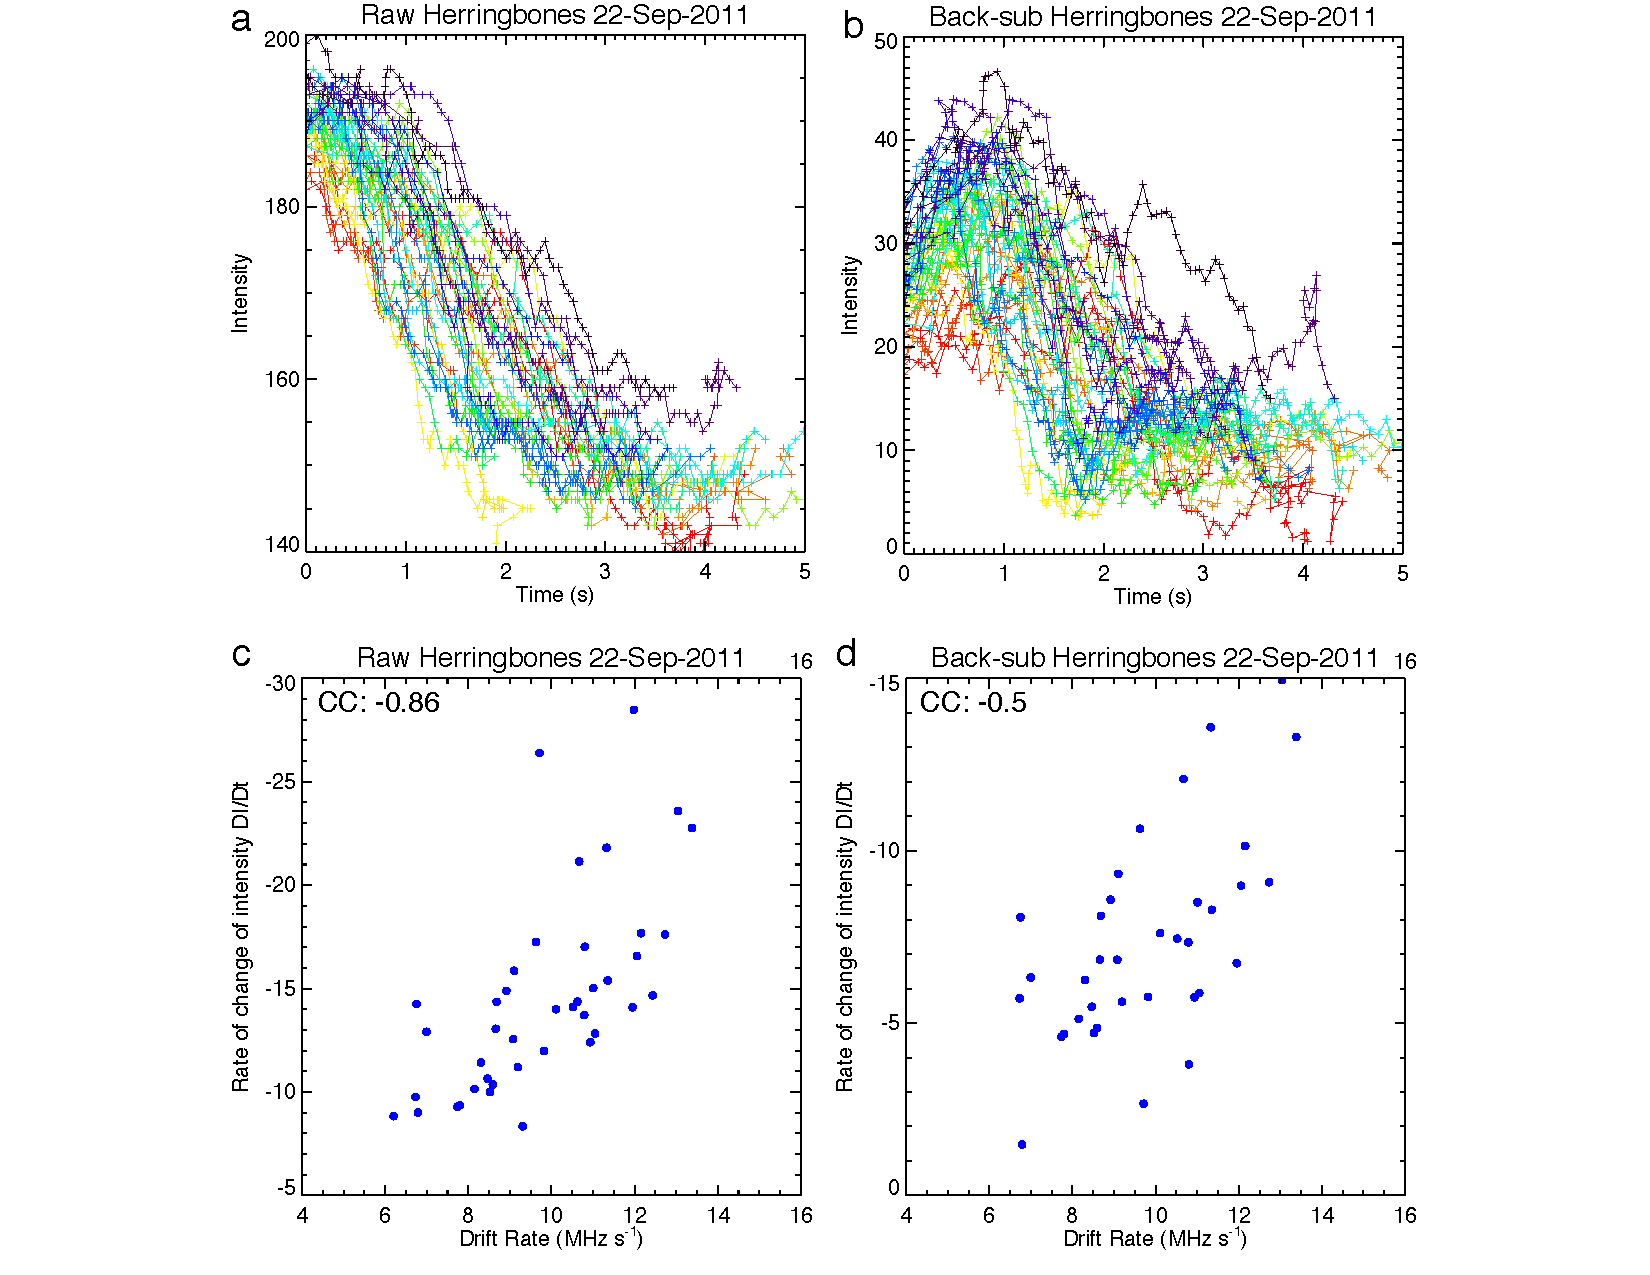
\includegraphics[scale=0.7, trim=3.5cm 0cm 0cm 1cm]{herringbone_stats2.pdf}
\caption[Hough transform herringbones]{(a) Intensity versus time for raw data; (b) intensity versus time for background subtracted data. (c) and (d) show scatter plots of drift rate versus rate of change of intensity along the burst for raw and background subtracted data, respectively.  The two show a good correlation which might suggest that the faster the beam, the faster it loses its energy}
\label{fig:bibt}
\end{center}
\end{figure}
Figure~\ref{fig:bibf}a and b shows the intensity as a function of frequency for all bursts for both raw data and background subtracted data (colours correspond to the individual bursts in Figure~\ref{fig:hough_hb}). Overall the intensity increases for bursts later in the sequence (increase in intensity form red to purple), which is a general feature of the bursts in the original spectra. The background subtracted data also reveals a peak at $\sim$45\,MHz, which may be interpreted as the start frequency of these features.
Figure~\ref{fig:bibf}b and c shows the frequency with respect to time for all bursts, with each showing a linear trend and range from $\sim$5--13\,MHz\,s$^{-1}$.
\begin{figure}[t!]
\begin{center}
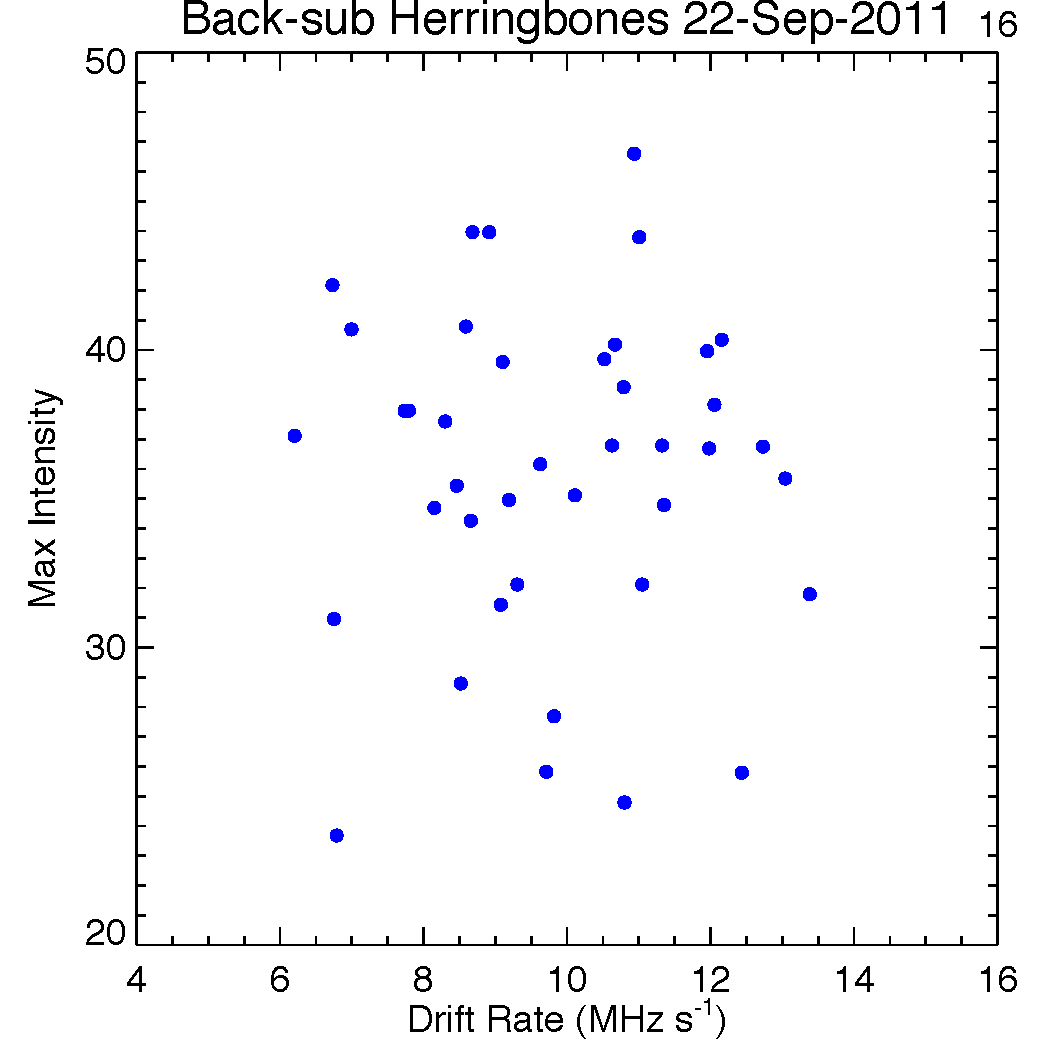
\includegraphics[scale=0.5, trim=1.5cm 0cm 0cm 1cm]{hough_maxi.pdf}
\caption[Hough transform herringbones]{Scatter plot of drift rate and maximum intensity of the burst. They show no correlation despite the fact Equation~\ref{eqn:plasma_emiss} would imply that they should. A larger data set needs to be explored in order to investigate this.}
\label{fig:maxi}
\end{center}
\end{figure}
The intensity with respect to time is shown in Figure~\ref{fig:bibt}a and b, revealing much of the same characteristics as Figure~\ref{fig:bibf}a and b. An interesting correlation is shown in Figure~\ref{fig:bibt}b and c. The drift rate shows a negative correlation with the rate of change of intensity of the bursts. This may be interpreted as the faster the electron beams travel, the quicker they lose their energy and induce radiation for a shorter amount of time. This would agree with Equation~\ref{eqn:plasma_emiss}, which highlights the relationship between plasma emission emissivity and beam velocity.  Despite the fact that there seems to be a correlation between the two parameters, there are a low number of data points and more bursts need to be included into the statistics if anything meaningful can be extracted from these results. Surprisingly, the maximum intensity and the drift rate do not show any correlation (Figure~\ref{fig:maxi}), which would be expected from Equation~\ref{eqn:plasma_emiss}. Again, this might be a symptom of low number statistics and needs to be further investigated.
%
%

As can be seen in Figure~\ref{fig:hough_hb}, the Hough transform is not perfect, and may miss some of the weaker or more patchy bursts. A greater effort needs to be made to ensure transform picks up the burst on the finest scales. One approach could be to use gradients to highlight edges in the image before using the Hough transform. A more sophisticated technique could be through multi-scale filtering using wavelets, this could highlight only the bursts, allowing the Hough transform to detect the smaller and fainter bursts more easily.

A statistical study of herringbone features has been lacking in recent times and a modern approach would compliment the herringbone statistical analysis of \citep{cairns1987, mann1995}. Is is still an unknown as to why some type IIs exhibit herringbones and why some do not. Future studies employing multi wavelength analysis, such as Carley {\it et al.}\,(2013), combined with a statistical analysis like the one presented in this section, can reveal both what caused the herringbones and what is the nature of the particle acceleration. Further analysis comparing emissivities and particle drift rates may reveal some details of the plasma emission mechanism.

%\subsubsection{100 CME Challenge}


